\chapter{Graph Algorithms}
\label{chapter:graph}

\abstract{
We have seen two major classes of algorithms that approach the top-$k$ retrieval
problem in their own unique ways. One recursively partitions a vector collection to model its
geometry, and the other hashes the vectors into predefined buckets to reduce the search space.
Our next class of algorithms takes yet a different view of the question.
At a high level, our third approach is to ``walk'' through a collection,
hopping from one vector to another, where every hop
gets us \emph{spatially} closer to the optimal solution.
This chapter reviews algorithms that use a graph data structure
to implement that idea.
}

\section{Intuition}
\label{section:graph:intuition}

The most natural way to understand a spatial walk through a collection
of vectors is by casting it as traversing a (directed) connected graph.
As we will see, whether the graph is directed or not depends on the specific algorithm itself.
But the graph must regardless be \emph{connected}, so that there always exists at least
one path between every pair of nodes. This ensures that we can walk through the graph
no matter where we begin our traversal.

Let us write $G(\mathcal{V}, \mathcal{E})$ to refer to such a graph,
whose set of \emph{vertices} or \emph{nodes} are denoted by $\mathcal{V}$,
and its set of edges by $\mathcal{E}$.
So, for $u, v \in \mathcal{V}$ in a directed graph,
if $(u, v) \in \mathcal{E}$, we may freely move from node $u$ to node $v$.
Hopping from $v$ to $u$ is not possible if $(v, u) \notin \mathcal{E}$.
Because we often need to talk about the set of nodes that can be reached by a single hop
from a node $u$---known as the neighbors of $u$---we give it a special symbol and
define that set as follows: $N(u) = \{ v \;|\; (u, v) \in \mathcal{E} \}$.

The idea behind the algorithms in this chapter is to construct a graph in the pre-processing phase
and use that as an index of a vector collection for top-$k$ retrieval.
To do that, we must decide what is a node in the graph (i.e., define the set $\mathcal{V}$),
how nodes are linked to each other ($\mathcal{E}$), and, importantly, what the search algorithm looks like.

\smallskip

The set of nodes $\mathcal{V}$ is easy to construct:
Simply designate every vector in the collection $\mathcal{X}$
as a unique node in $G$, so that $\lvert \mathcal{X} \rvert = \lvert \mathcal{V} \rvert$.
There should, therefore, be no ambiguity if we referred to a node
as a vector. We use both terms interchangeably.

What properties should the edge set $\mathcal{E}$ have?
To get a sense of what is required of the edge set,
it would help to consider the search algorithm first.
Suppose we are searching for the top-$1$ vector closest to query $q$,
and assume that we are, at the moment, at an arbitrary node $u$ in $G$.

From node $u$, we can have a look around and assess if any of our neighbors
in $N(u)$ is closer to $q$. By doing so, we find ourselves in one of two situations.
Either we encounter no such neighbor, so that $u$ has the smallest
distance to $q$ among its neighbors. If that happens, ideally, we want $u$ to also have
the smallest distance to $q$ among \emph{all} vectors. In other words, in an ideal graph,
a local optimum coincides with the global optimum.

\begin{figure}[t]
    \centering
    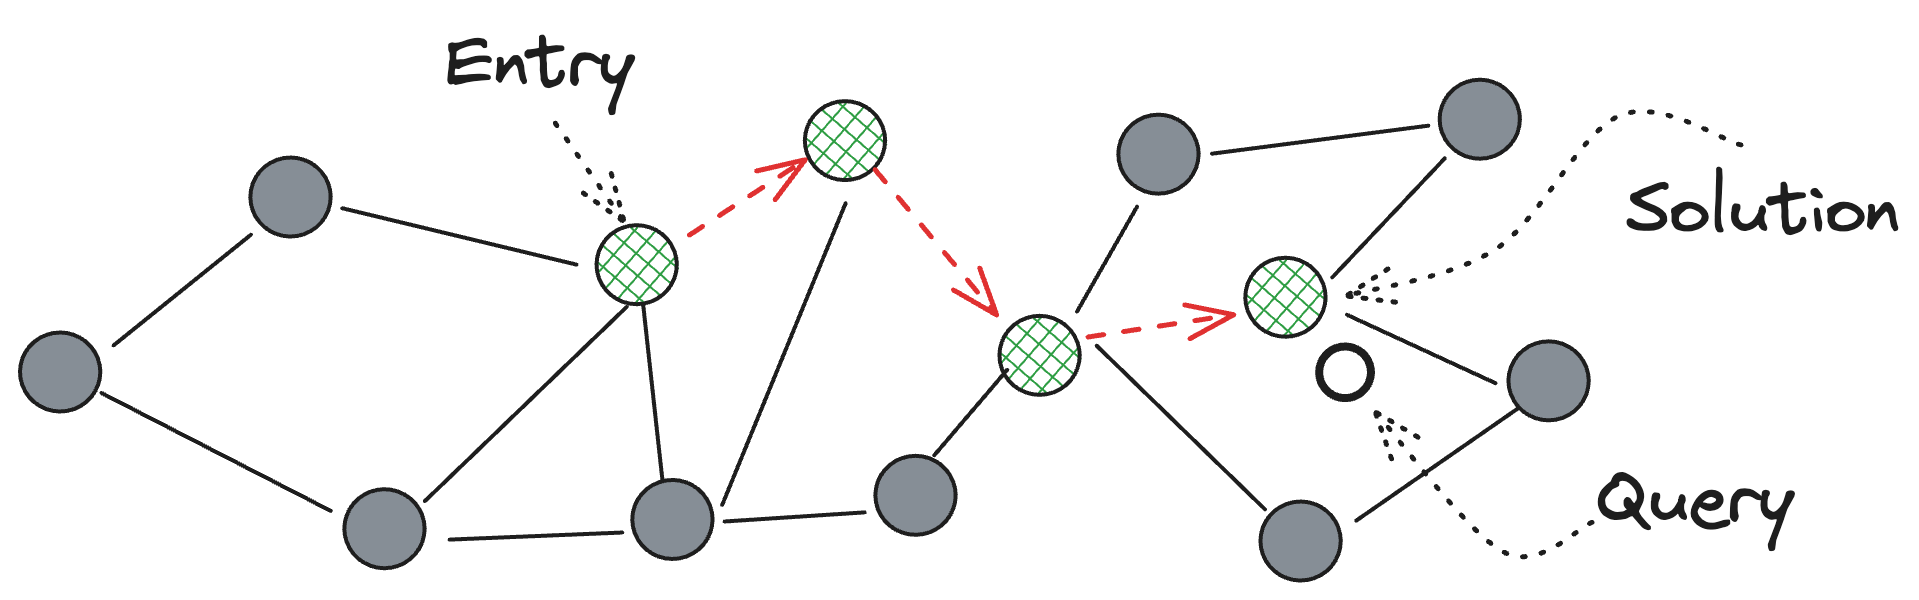
\includegraphics[width=0.7\linewidth]{figures/graphs-greedy-traversal.png}
    \caption{Illustration of the greedy traversal algorithm for finding
    the top-$1$ solution on an example (undirected) graph. The procedure enters
    the graph from an arbitrary ``entry'' node. It then compares the distance of the node to query $q$
    with the distance of its neighbors to $q$, and either terminates if no neighbor is closer
    to $q$ than the node itself, or advances to the closest neighbor. It repeats this procedure
    until the terminal condition is met. The research question in
    this chapter concerns the construction of the edge set: How do we construct a sparse graph
    which can be traversed greedily while providing guarantees on the (near-)optimality
    of the solution}
    \label{figure:graphs:greedy-traversal}
\end{figure}

Alternatively, we may find one such neighbor $v \in N(u)$ for which $\delta(q, v) < \delta(q, u)$
and $v = \argmin_{w \in N(u)} \delta(q, w)$.
In that case, the ideal graph is one where the following event takes place: If we moved from
$u$ to $v$, and repeated the process above in the context of $N(v)$ and so on, we will ultimately
arrive at a local optimum (which, by the previous condition, is the global optimum).
Terminating the algorithm then would therefore give us the optimal solution to the
top-$1$ retrieval problem.

\begin{svgraybox}
Put differently, in an ideal graph, if moving from a node to any of its neighbors
does not get us spatially closer to $q$, it is because the current
node is the optimal solution to the top-$1$ retrieval problem for $q$.
\end{svgraybox}

On a graph with that property,
the procedure of starting from any node in the graph,
hopping to a neighbor that is closer to $q$, and repeating this procedure until no such neighbor
exists, gives the optimal solution.
That procedure is the familiar \emph{best-first-search} algorithm,
which we illustrate on a toy graph in Figure~\ref{figure:graphs:greedy-traversal}.
That will be our base search algorithm for top-$1$ retrieval.

\begin{algorithm}[!t]
\SetAlgoLined
{\bf Input: }{Graph $G=(\mathcal{V}, \mathcal{E})$ over collection $\mathcal{X}$ 
with distance $\delta(\cdot, \cdot)$; query point $q$; entry node $s \in \mathcal{V}$;
retrieval depth $k$.}\\
\KwResult{Exact top-$k$ solution for $q$.}

\begin{algorithmic}[1]

\STATE $Q \leftarrow \{ s \}$ \Comment*[l]{\footnotesize $Q$ is a priority queue}

\WHILE{$Q$ changed in the previous iteration}
    \STATE $\mathcal{S} \leftarrow \bigcup_{u \in Q} N(u)$
    \STATE $v \leftarrow \argmin_{u \in \mathcal{S}} \delta(q, u)$

    \STATE $Q.\textsc{Insert}(v)$
    \IF{$\lvert Q \rvert \geq k$}
        \STATE $Q.\textsc{Pop}()$ \Comment*[l]{\footnotesize Removes the node with the largest distance to $q$}
    \ENDIF
\ENDWHILE

\RETURN $Q$
\end{algorithmic}
\caption{Greedy search algorithm for top-$k$ retrieval over a graph index.}
\label{algorithm:graphs:greedy-search}
\end{algorithm}

Extending the search algorithm to top-$k$ requires a minor modification to the procedure above.
It begins by initializing a priority queue of size $k$. When we visit a new node, we add it to
the queue if its distance with $q$ is smaller than the minimum distance among the nodes already in the queue.
We keep moving from a node in the queue to its neighbors until the queue stabilizes (i.e., no
unseen neighbor of any of the nodes in the queue has a smaller distance to $q$).
This is described in Algorithm~\ref{algorithm:graphs:greedy-search}.

Note that, assuming $\delta(\cdot, \cdot)$ is proper, it is easy to see that
the top-$1$ optimality guarantee immediately implies top-$k$
optimality---you should verify this claim as an exercise.
It therefore suffices to state our requirements in terms of top-$1$ optimality alone.
So, ideally, $\mathcal{E}$ should guarantee that traversing $G$
in a best-first-search manner yields the optimal top-$1$ solution.

\subsection{The Research Question}

It is trivial to construct an edge set that provides the desired optimality guarantee:
Simply add an edge between every pair of nodes, completing the graph!
The greedy search algorithm described above will take us to the optimal solution.

However, such a graph not only has high space complexity, but it also has a linear query time complexity.
That is because, the very first step (which also happens to be the last step)
involves comparing the distance of $q$ to the entry node,
with the distance of $q$ to every other node in the graph! We are better off exhaustively
scanning the entire collection in a flat index.

\begin{svgraybox}
The research question that prompted the algorithms we are about to study in this chapter is
whether there exists a relatively \emph{sparse} graph that has the optimality guarantee we seek
or that can instead provide guarantees for the more relaxed,
$\epsilon$-approximate top-$k$ retrieval problem.
\end{svgraybox}

As we will learn shortly, with a few notable exceptions,
all constructions of $\mathcal{E}$ proposed thus far in the literature 
for high-dimensional vectors amount to
heuristics that attempt to \emph{approximate} a theoretical graph but
come with no guarantees. In fact, in almost all cases,
their worst-case complexity is no better than exhaustive search.
Despite that, many of these heuristics work remarkably well
in practice on real datasets, making graph-based methods one of the most
widely adopted solutions to the approximate top-$k$ retrieval problem.

\smallskip

In the remainder of this chapter, we will see classes of theoretical graphs
that were developed in adjacent scientific disciplines, but that are seemingly suitable
for the (approximate) top-$k$ retrieval problem. As we introduce these graphs,
we also examine representative algorithms that aim to build an approximation
of such graphs in high dimensions, and review their properties.

We note, however, that the literature on graph-based methods is vast and growing still.
There is a plethora of studies that experiment with (minor or major) adjustments to the basic idea
described earlier, or that empirically compare and contrast different algorithmic flavors
on real-world datasets.
This chapter does not claim to, nor does it intend to cover the explosion of
material on graph-based algorithms. Instead, it limits its scope to the foundational
principles and ground-breaking works that are theoretically somewhat interesting.
We refer the reader to existing reports and surveys for the full spectrum of
works on this topic~\citep{wang2021survey-graph-ann,li2020survey-ann}.

\section{The Delaunay Graph}
One classical graph that satisfies the conditions we seek and guarantees the optimality
of the solution obtained by best-first-search traversal
is the Delaunay graph~\citep{Delaunay_1934aa,fortune1997voronoi}.
It is easier to understand the construction of the Delaunay graph if we consider instead
its dual: the Voronoi diagram. So we begin with a description of the Voronoi diagram and
Voronoi regions.

\subsection{Voronoi Diagram}

For the moment, suppose $\delta$ is the Euclidean distance and that we are in $\mathbb{R}^2$.
Suppose further that we have a collection $\mathcal{X}$ of just two points $u$ and $v$
on the plane.
Consider now the subset of $\mathbb{R}^2$ comprising of all the points
to which $u$ is the closest point from $\mathcal{X}$.
Similarity, we can identify the subset to which $v$ is the closest point.
These two subsets are, in fact, partitions of the plane and are separated by a
line---the points on this line are equidistant to $u$ and $v$.
In other words, two points in $\mathbb{R}^2$ induce a partitioning of 
the plane where each partition is ``owned'' by a point and describes the
set of points that are closer to it than they are to the other point.

\begin{figure}[t]
    \centering
    \subfloat[Voronoi diagram]{
        \label{figure:graphs:delaunay:voronoi}
        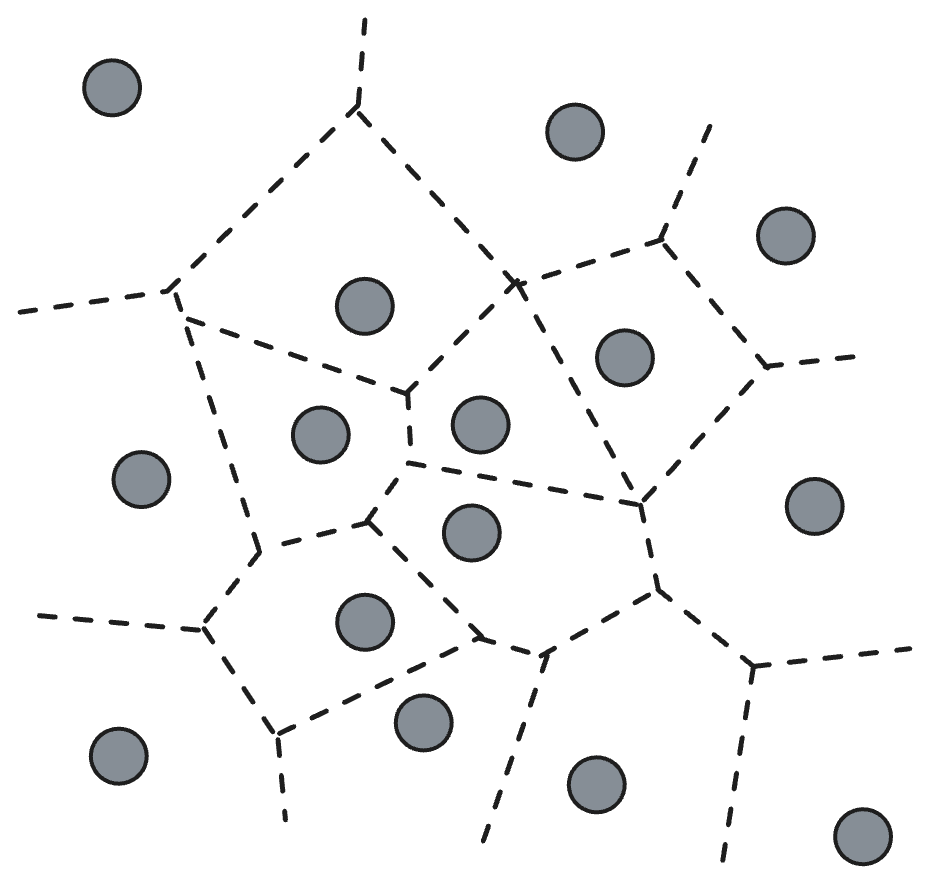
\includegraphics[width=0.33\linewidth]{figures/graphs-voronoi-diagram.png}
    }
    \subfloat[Delaunay graph]{
        \label{figure:graphs:delaunay:graph}
        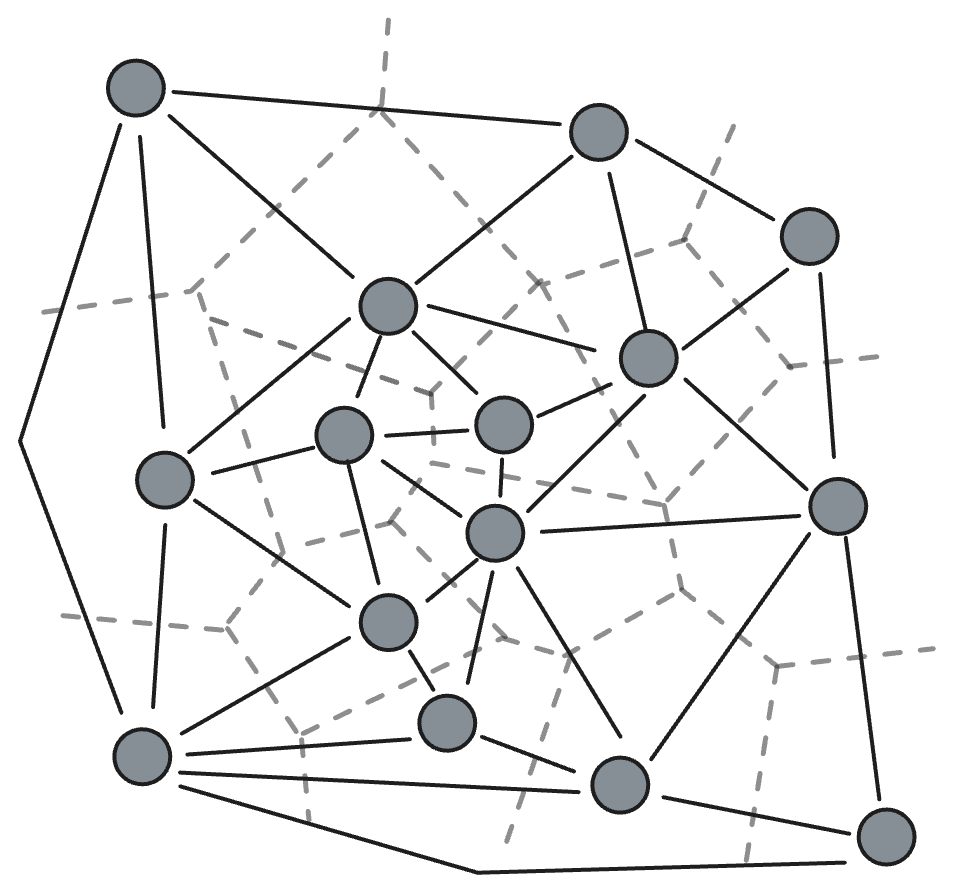
\includegraphics[width=0.33\linewidth]{figures/graphs-delaunay-graph-overlay.png}
    }
    \caption{Visualization of the Voronoi diagram (a) and its dual, the Delaunay graph (b)
    for an example collection $\mathcal{X}$ of points in $\mathbb{R}^2$.
    A Voronoi region associated with a point $u$
    (shown here as the area contained within the dashed lines)
    is a set of points whose nearest neighbor in $\mathcal{X}$
    is $u$. The Delaunay graph is an undirected graph whose nodes are points in $\mathcal{X}$ and two nodes
    are connected (shown as solid lines) if their Voronoi regions have a non-empty intersection.}
    \label{figure:graphs:delaunay}
\end{figure}

We can trivially generalize that notion to more than two points and, indeed, to higher dimensions.
A collection $\mathcal{X}$ of points in $\mathbb{R}^d$ partitions the space
into unique regions $\mathcal{R} = \bigcup_{u \in \mathcal{X}} \mathcal{R}_u$,
where the region $\mathcal{R}_u$ is owned by point
$u \in \mathcal{X}$ and represents the set of points to which $u$ is the closest
point in $\mathcal{X}$. Formally, $\mathcal{R}_u = \{ x \;|\; u = \argmin_{v \in \mathcal{X}} \delta(x, v) \}$. Note that, each region is a convex polytope that is the intersection of
half-spaces.
The set of regions is known as the Voronoi diagram for the collection $\mathcal{X}$ and is
illustrated in Figure~\subref*{figure:graphs:delaunay:voronoi} for an example collection in $\mathbb{R}^2$.

\subsection{Delaunay Graph}

The Delaunay graph for $\mathcal{X}$ is, in effect, a graph representation of its
Voronoi diagram.
The nodes of the graph are trivially the points in $\mathcal{X}$, as before.
We place an edge between two nodes $u$ and $v$ if their Voronoi regions have a non-empty
intersection: $\mathcal{R}_u \cap \mathcal{R}_v \neq \emptyset$. Clearly, by construction,
this graph is undirected. An example
of this graph is rendered in Figure~\subref*{figure:graphs:delaunay:graph}.

\medskip 

There is an important technical detail that is worth noting.
The Delaunay graph for a collection $\mathcal{X}$ is unique if the points
in $\mathcal{X}$ are in \emph{general position}~\citep{fortune1997voronoi}.
A collection of points are said to be in general position if the following two
conditions are satisfied. First, no $n$ points from $\mathcal{X} \subset \mathbb{R}^d$,
for $2 \leq n \leq d + 1$, must lie on a $(n-2)$-flat. Second, no $n+1$ points
must lie on any $(n-2)$-dimensional hypersphere. In $\mathbb{R}^2$, as an example,
for a collection of points to be in general position,
no three points may be co-linear, and no four points co-circular.

We must add that, the detail above is generally satisfied in practice.
Importantly, if the vectors in our collection are
independent and identically distributed, then the collection is almost surely in general
position. That is why we often take that technicality for granted.
So from now on, we assume that the Delaunay graph of a collection of points is unique.

\subsection{Top-\texorpdfstring{$1$}{1} Retrieval}
We can immediately recognize the importance of Voronoi regions: They geometrically
capture the set of queries for which a point from the collection is the solution
to the top-$1$ retrieval problem. But what is the significance of the dual representation
of this geometrical concept? How does the Delaunay graph help us solve the top-$1$
retrieval problem?

For one, the Delaunay graph is a compact representation of the Voronoi diagram.
Instead of describing polytopes, we need only to record edges between neighboring nodes.
But, more crucially, as the following claim shows, we can traverse the Delaunay graph greedily,
and reach the optimal top-$1$ solution from any node. In other words, the Delaunay graph
has the desired property we described in Section~\ref{section:graph:intuition}.

\begin{theorem}
    \label{theorem:graphs:delaunay}
    Let $G = (\mathcal{V}, \mathcal{E})$ be a graph that contains the Delaunay graph of $m$ vectors
    $\mathcal{X} \subset \mathbb{R}^d$.
    The best-first-search algorithm over $G$ gives the optimal solution to the top-$1$ retrieval problem
    for any arbitrary query $q$ if $\delta(\cdot, \cdot)$ is proper.
\end{theorem}

The proof of the result above relies on an important property of the Delaunay graph,
which we state first.

\begin{lemma}
\label{lemma:graphs:delaunay}
    Let $G = (\mathcal{V}, \mathcal{E})$ be the Delaunay graph of
    a collection of points $\mathcal{X} \subset \mathbb{R}^d$,
    and let $B$ be a ball centered at $\mu$ that contains two
    points $u, v \in \mathcal{X}$, with radius $r = \min (\delta(\mu, u), \delta(\mu, v))$,
    for a continuous and proper distance function $\delta(\cdot, \cdot)$.
    Then either $(u, v) \in \mathcal{E}$ or there exists a third point in $\mathcal{X}$
    that is contained in $B$.
\end{lemma}
\begin{proof}
Suppose there is no other point in $\mathcal{X}$ that is contained in $B$.
We must show that, in that case, $(u, v) \in \mathcal{E}$.

There are two cases.
The first and easy case is when $u$ and $v$ are on the surface of $B$.
Clearly, $u$ and $v$ are equidistant from $\mu$.
Because there are no other points in $B$,
we can conclude that $\mu$ lies in the intersection of $\mathcal{R}_u$
and $\mathcal{R}_v$, the Voronoi regions associated with $u$ and $v$.
That implies $(u, v) \in \mathcal{E}$.

\begin{figure}[t]
    \centering
    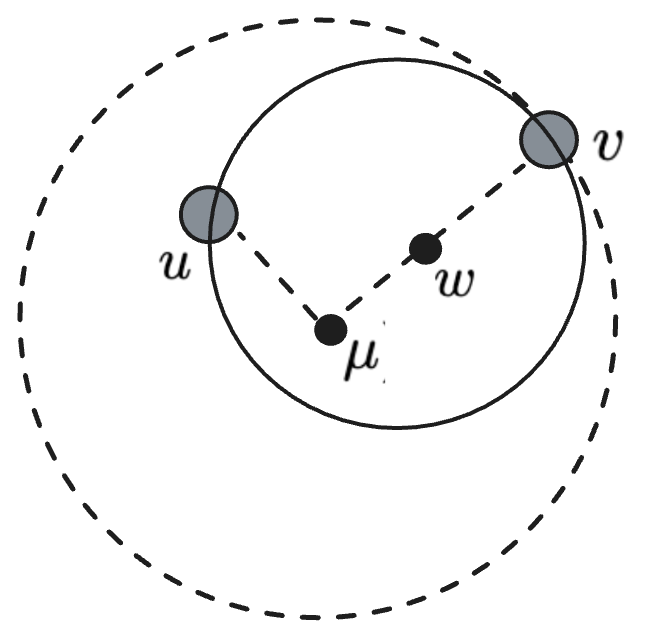
\includegraphics[width=0.25\linewidth]{figures/graphs-delaunay-proof-lemma.png}
    \caption{Illustration of the second case in the proof of Lemma~\ref{lemma:graphs:delaunay}.}
    \label{figure:graphs:delaunay:proof-lemma}
\end{figure}

In the second case, suppose $\delta(\mu, u) < \delta(\mu, v)$, so that $v$ is on the surface of $B$
and $u$ is in its interior. Consider the function
$f(\omega) = \delta(v, \omega) - \delta(u, \omega)$.
Clearly, $f(v) < 0$ and $f(\mu) > 0$. Therefore, there must be a point $w \in B$
on the line segment $\mu + \lambda (v - \mu)$ for $\lambda \in [0, 1]$ for which
$f(w) = 0$. That implies that $\delta(w, u) = \delta(w, v)$.
Furthermore, $v$ is the closest point on the surface of $B$ to $w$,
so that the ball centered at $w$ with radius $\delta(w, v)$ is entirely contained
in $B$. This is illustrated in Figure~\ref{figure:graphs:delaunay:proof-lemma}.

Importantly, no other point in $\mathcal{X}$ is closer to $w$ than $u$ and $v$.
So $w$ rests in the intersection of $\mathcal{R}_u$ and $\mathcal{R}_v$, and
$(u, v) \in \mathcal{E}$.
\end{proof}

\begin{proof}[Proof of Theorem~\ref{theorem:graphs:delaunay}]
    We prove the result for the case where $\delta$ is the Euclidean
    distance and leave the proof of the more general case as an exercise.
    (Hint: To prove the general case you should make the line segment
    argument as in the proof of Lemma~\ref{lemma:graphs:delaunay}.)

    Suppose the greedy search for $q$ stops at some local optimum $u$
    that is different from the global optimum, $u^\ast$,
    and that $(u, u^\ast) \notin \mathcal{E}$---otherwise,
    the algorithm must terminate at $u^\ast$ instead.
    Let $r = \delta(q, u)$.
    
    By assumption we have that the ball centered at $q$ with radius $r$,
    $B(q, r)$, is non-empty because it must contain $u^\ast$ whose distance to $q$ is less than $r$.
    Let $v$ be the point in this ball that is closest to $u$.
    Consider now the ball $B((u + v)/2, \delta(u, v)/2)$.
    This ball is empty: otherwise $v$ would not be the closest point to $u$.
    By Lemma~\ref{lemma:graphs:delaunay}, we must have that $(u, v) \in \mathcal{E}$.
    This is a contradiction because the greedy search cannot stop at $u$.
\end{proof}

\begin{svgraybox}
Notice that Theorem~\ref{theorem:graphs:delaunay} holds for any graph
that \emph{contains} the Delaunay graph.
The next theorem strengthens this result to show that the Delaunay graph represents
the minimal edge set that guarantees an optimal solution through greedy traversal.
\end{svgraybox}

\begin{theorem}
    \label{theorem:graphs:delaunay-is-minimal}
    The Delaunay graph is the minimal graph over which the best-first-search algorithm
    gives the optimal solution to the top-$1$ retrieval problem.
\end{theorem}

In other words, if a graph does not contain the Delaunay graph, then we can find queries
for which the greedy traversal from an entry point does not produce the optimal top-$1$
solution.

\begin{proof}[Proof of Theorem~\ref{theorem:graphs:delaunay-is-minimal}]
    Suppose that the data points $\mathcal{X}$ are in general position.
    Suppose further that $G = (\mathcal{V}, \mathcal{E})$ is a graph built from $\mathcal{X}$,
    and that $u$ and $v$ are two nodes in the graph.
    Suppose further that $(v, u) \notin \mathcal{E}$ but that that edge
    exists in the Delaunay graph of $\mathcal{X}$.

    If we could sample a query point $q$ such that
    $\delta(q, u) < \delta(q, v)$ but 
    $\delta(q, w) > \max(\delta(q, u), \delta(q, v))$ for all $w \neq u, v$,
    then we are done.
    That is because, if we entered the graph through $v$, then $v$ is a local optimum
    in its neighborhood: all other points that are connected to $v$ have a distance larger than $\delta(q, v)$.
    But $v$ is not the globally optimal solution, so that the greedy traversal does not converge to the
    optimal solution.

    It remains to show that such a point $q$ always exists.
    Suppose it did not. That is, for any point that is in the Voronoi region of $u$,
    there is a data point $w \neq v$ that is closer to it than $v$.
    If that were the case, then no ball whose boundary passes through $u$ and $v$
    can be empty, which contradicts Lemma~\ref{lemma:graphs:delaunay} (the ``empty-circle''
    property of the Delaunay graph).
\end{proof}

As a final remark on the Delaunay graph and its use in top-$1$ retrieval, we note that
the Delaunay graph only makes sense if we have precise knowledge of the structure of the space
(i.e., the metric). It is not enough to have just pairwise distances between points in a collection
$\mathcal{X}$. In fact,~\cite{navarro2002spatial-approximateion} showed that if pairwise
distances are all we know about a collection of points, then the only sensible
graph that contains the Delaunay graph and is amenable to greedy search is the complete graph.
This is stated as the following theorem.

\begin{theorem}
    Suppose the structure of the metric space is unknown, but we have pairwise distances between
    the points in a collection $\mathcal{X}$, due to an arbitrary, but proper distance function $\delta$.
    For every choice of $u, v \in \mathcal{X}$,
    there is a choice of the metric space such that $(u, v) \in \mathcal{E}$,
    where $G = (\mathcal{V}, \mathcal{E})$ is a Delaunay graph for $\mathcal{X}$.
\end{theorem}
\begin{proof}
    The idea behind the proof is to assume $(u, v) \notin \mathcal{E}$, then
    construct a query point that necessitates the existence of an edge between $u$ and $v$.
    To that end, consider a query point $q$ such that its distance to $u$ is $C + \epsilon$ for some
    constant $C$ and $\epsilon > 0$, its distance to $v$ is $C$, and its distance to 
    every other point in $\mathcal{X}$ is $C + 2 \epsilon$.

    This is a valid arrangement if we choose $\epsilon$ such that
    $\epsilon \leq 1/2 \min_{x, y \in \mathcal{X}} \delta(x, y)$
    and $C$ such that $C \geq 1/2 \max_{x, y \in \mathcal{X}} \delta(x, y)$. It is easy to verify that,
    if those conditions hold, a point $q$ with the prescribed distances can exist as the distances
    do not violate any of the triangle inequalities.

    Consider then a search starting from node $u$. If $(u, v) \notin \mathcal{E}$, then for the search
    algorithm to walk from $u$ to the optimal solution, $v$, it must first get \emph{farther} from $q$.
    But we know by the properties of the Delaunay graph that such an event implies that
    $u$ (which would be the local optimum) must be the global optimum. That is clearly not true.
    So we must have that $(u, v) \in \mathcal{E}$, giving the claim.
\end{proof}

\subsection{Top-\texorpdfstring{$k$}{k} Retrieval}

Let us now consider the general case of top-$k$ retrieval over the Delaunay graph.
The following result states that Algorithm~\ref{algorithm:graphs:greedy-search} is correct
if executed on any graph that contains the Delaunay graph, in the sense that it returns the
optimal solution to top-$k$ retrieval.

\begin{theorem}
    \label{theorem:graphs:delaunay:top-k}
    Let $G = (\mathcal{V}, \mathcal{E})$ be a graph that contains the Delaunay graph of $m$ vectors
    $\mathcal{X} \subset \mathbb{R}^d$.
    Algorithm~\ref{algorithm:graphs:greedy-search} over $G$ gives the optimal solution to the top-$k$ retrieval problem
    for any arbitrary query $q$ if $\delta(\cdot, \cdot)$ is proper.
\end{theorem}
\begin{proof}
    As with the proof of Theorem~\ref{theorem:graphs:delaunay},
    we show the result for the case where $\delta$ is the Euclidean
    distance and leave the proof of the more general case as an exercise.
    
    The proof is similar to the proof of Theorem~\ref{theorem:graphs:delaunay} but the argument
    needs a little more care when $k > 1$.
    Suppose Algorithm~\ref{algorithm:graphs:greedy-search} for $q$ stops at some local optimum set
    $Q$ that is different from the global optimum, $Q^\ast$. In other words,
    $Q \;\triangle\; Q^\ast \neq \emptyset$ where $\triangle$ denotes the symmetric difference between
    sets.

    Let $r = \max_{u \in Q} \delta(q, u)$ and consider the ball $B(q, r)$.
    Because $Q \;\triangle\; Q^\ast \neq \emptyset$, there must be at least $k$ points in the interior of this ball.
    Let $v \notin Q$ be a point in the interior and suppose $u \in Q$ is its closest point in the ball.
    Clearly, the ball $B((u + v)/2, \delta(u, v)/2)$ is empty:
    otherwise $v$ would not be the closest point to $u$.
    By Lemma~\ref{lemma:graphs:delaunay}, we must have that $(u, v) \in \mathcal{E}$.
    This is a contradiction because Algorithm~\ref{algorithm:graphs:greedy-search} would, before termination,
    place $v$ in $Q$ to replace the node that is on the surface of the ball.
\end{proof}

\subsection{The \texorpdfstring{$k$}{k}-NN Graph}

From our discussion of Voronoi diagrams and Delaunay graphs, it appears as though we have
found the graph we have been looking for. Indeed, the Delaunay graph of a collection of vectors
gives us the exact solution to top-$k$ queries, using such a strikingly simple search algorithm.
Sadly, the story does not end there and, as usual,
the relentless curse of dimensionality poses a serious challenge.

The first major obstacle in high dimensions actually concerns
the construction of the Delaunay graph itself. While there are many
algorithms~\citep{edelsbrunner1992delaunay,guibas1992delaunay,guibas1985voronoi}
that can be used to construct the Delaunay graph---or, to be more precise,
to perform Delaunay \emph{triangulation}---all suffer from an exponential dependence
on the number of dimensions $d$. So building the graph itself seems infeasible when $d$
is too large.

\begin{figure}[t]
    \centering
    \subfloat[Delaunay graph]{
        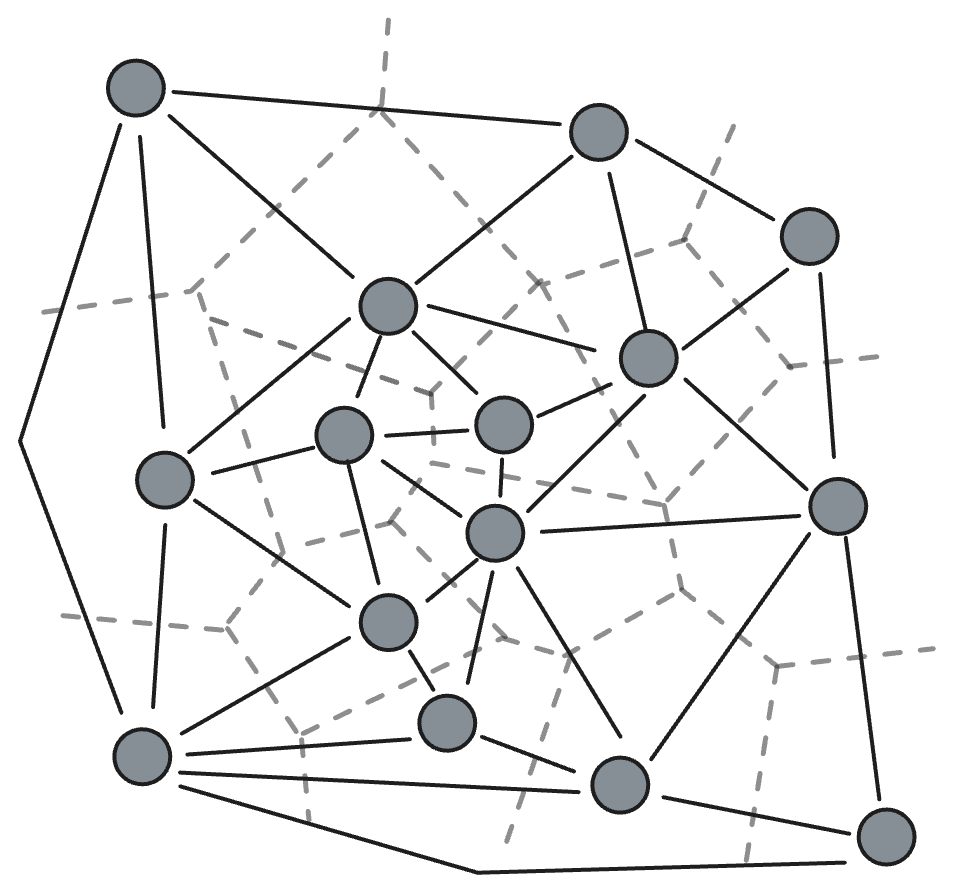
\includegraphics[width=0.33\linewidth]{figures/graphs-delaunay-graph-overlay.png}
    }
    \subfloat[$2$-NN graph]{
        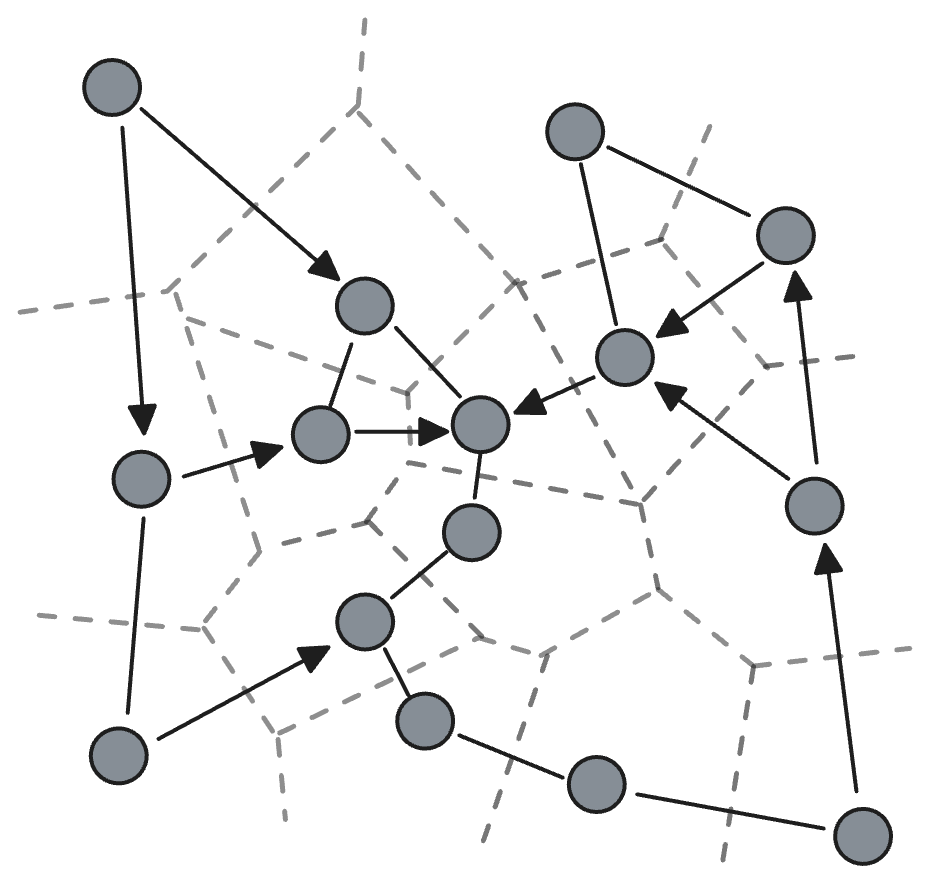
\includegraphics[width=0.33\linewidth]{figures/graphs-delaunay-knn.png}
    }
    \caption{Comparison of the Delaunay graph (a) with the $k$-NN graph for $k=2$ (b)
    for an example collection in $\mathbb{R}^2$.
    In the illustration of the directed $k$-NN graph, edges that go in both directions
    are rendered as lines without arrow heads.
    Notice that, the top left node cannot be reached from the rest
    of the graph.}
    \label{figure:graphs:knn-graph}
\end{figure}

Even if we were able to quickly construct the Delaunay graph for a large collection of
points, we would face a second debilitating issue: The graph is close to complete!
While exact bounds on the expected number of edges in the graph surely depend on the data
distribution, in high dimensions the graph becomes necessarily more dense.
Consider, for example, vectors that are independent and identically-distributed
in each dimension. Recall from our discussion from Chapter~\ref{chapter:instability},
that in such an arrangement of points, the distance between any pair of points tends to
concentrate sharply. As a result, the Delaunay graph has an edge between almost every
pair of nodes.

\bigskip

These two problems are rather serious, rendering the guarantees of the Delaunay graph for
top-$k$ retrieval mainly of theoretical interest. These same difficulties motivated
research to \emph{approximate} the Delaunay graph. One prominent method is known
as the $k$-NN graph~\citep{chavez2010knn,hajebi2011fast,fu2016efanna}.

The $k$-NN graph is simply a $k$-regular graph where every node (i.e., vector) is
connected to its $k$ closest nodes. So $(u, v) \in \mathcal{E}$ if $v \in \argmin^{(k)}_{w \in \mathcal{X}} \delta(u, w)$. Note that, the resulting graph may be directed, depending on the choice of $\delta$.
We should mention, however, that researchers have explored ways of turning the $k$-NN graph
into an undirected graph~\citep{chavez2010knn}. An example is depicted in
Figure~\ref{figure:graphs:knn-graph}.

We must remark on two important properties of the $k$-NN graph.
First, the graph itself is far more efficient to construct than the Delaunay
graph~\citep{chen2009fast-knngraph-construction,vaidya1989knn-construction,connor2010fast-knngraph,dong2011knn-graph}.
The second point concerns the connectivity of the graph.
As \cite{Brito1997knn-graph} show, under mild conditions governing the distribution of the vectors
and with $k$ large enough, the resulting graph has a high probability of being connected.
When $k$ is too small, on the other hand, the resulting graph may become too sparse,
leading the greedy search algorithm to get stuck in local minima.

Finally, at the risk of stating the obvious, the $k$-NN graph does not enjoy any of
the guarantees of the Delaunay graph in the context of top-$k$ retrieval.
That is simply because the $k$-NN graph is likely only a sub-graph of the Delaunay graph,
while Theorems~\ref{theorem:graphs:delaunay} and~\ref{theorem:graphs:delaunay:top-k}
are provable only for super-graphs of the Delaunay graph.
Despite these deficiencies, the $k$-NN graph remains an important component
of advanced graph-based, approximate top-$k$ retrieval algorithms.

\subsection{The Case of Inner Product}
Everything we have stated so far about the Voronoi diagrams and its duality with
the Delaunay graph was contingent on $\delta(\cdot, \cdot)$ being proper.
In particular, the proof of the optimality guarantees implicitly require non-negativity
and the triangle inequality. As a result, none of the results apply to MIPS \emph{prima facie}.
As it turns out, however, we could extend the definition of Voronoi regions and the Delaunay graph
to inner product, and present guarantees for MIPS (with $k=1$, but not with $k>1$).
That is the proposal by \cite{morozov2018ip-nsw}.

\subsubsection{The IP-Delaunay Graph}
Let us begin by characterizing the Voronoi regions for inner product.
The Voronoi region $\mathcal{R}_u$ of a vector $u \in \mathcal{X}$ comprises of
the set of points for which $u$ is the maximizer of inner product:
\begin{equation*}
    \mathcal{R}_u = \{ x \in \mathbb{R}^d \;|\; u = \argmax_{v \in \mathcal{X}} \langle x, v \rangle \}.
\end{equation*}
This definition is essentially the same as how we defined the Voronoi region for a proper $\delta$,
and, indeed, the resulting Voronoi diagram is a partitioning of the whole space.
The properties of the resulting Voronoi regions, however, could not be more different.

First, recall from Section~\ref{section:flavors:flavors:mips} that inner product
does not even enjoy what we called coincidence. That is, in general, $u = \argmax_{v \in \mathcal{X}} \langle u, v \rangle$
is not guaranteed. So it is very much possible that $\mathcal{R}_u$ is empty for some
$u \in \mathcal{X}$. Second, when $\mathcal{R}_u \neq \emptyset$, it is a convex cone
that is the intersection of half-spaces that \emph{pass through the origin}. So the Voronoi
regions have a substantially different geometry. Figure~\subref*{figure:graphs:ip-delaunay:ip-voronoi}
visualizes this phenomenon.

\begin{figure}[t]
    \centering
    \subfloat[Euclidean Delaunay]{
        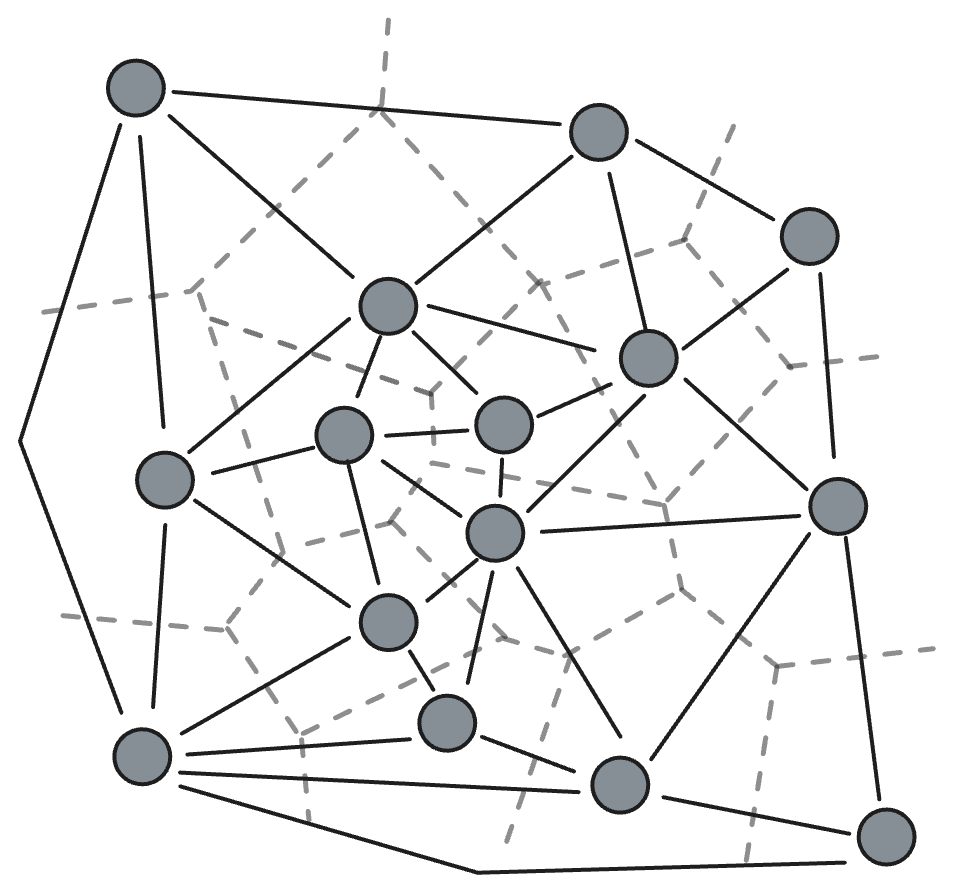
\includegraphics[width=0.32\linewidth]{figures/graphs-delaunay-graph-overlay.png}
    }
    \subfloat[Inner Product Voronoi]{
        \label{figure:graphs:ip-delaunay:ip-voronoi}
        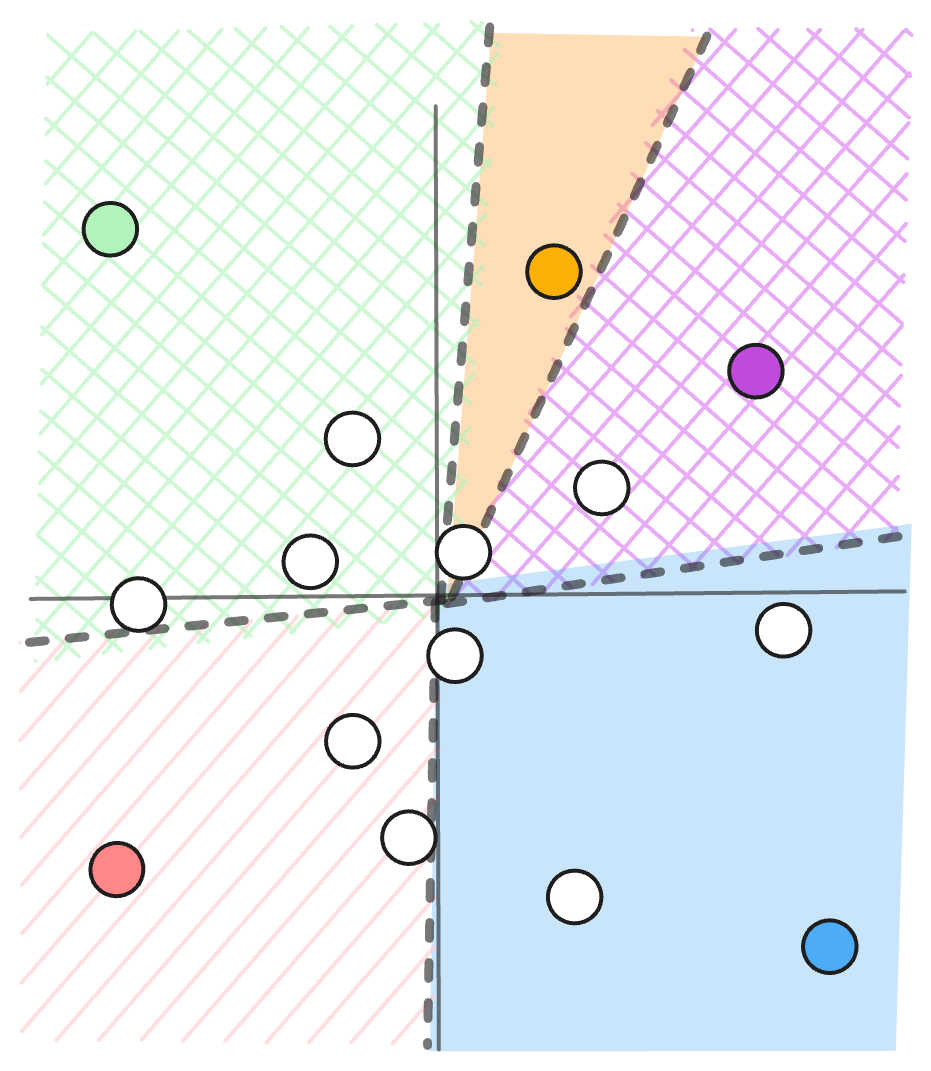
\includegraphics[width=0.32\linewidth]{figures/graphs-ip-voronoi-diagram.png}
    }
    \subfloat[IP-Delaunay]{
        \label{figure:graphs:ip-delaunay:ip-graph}
        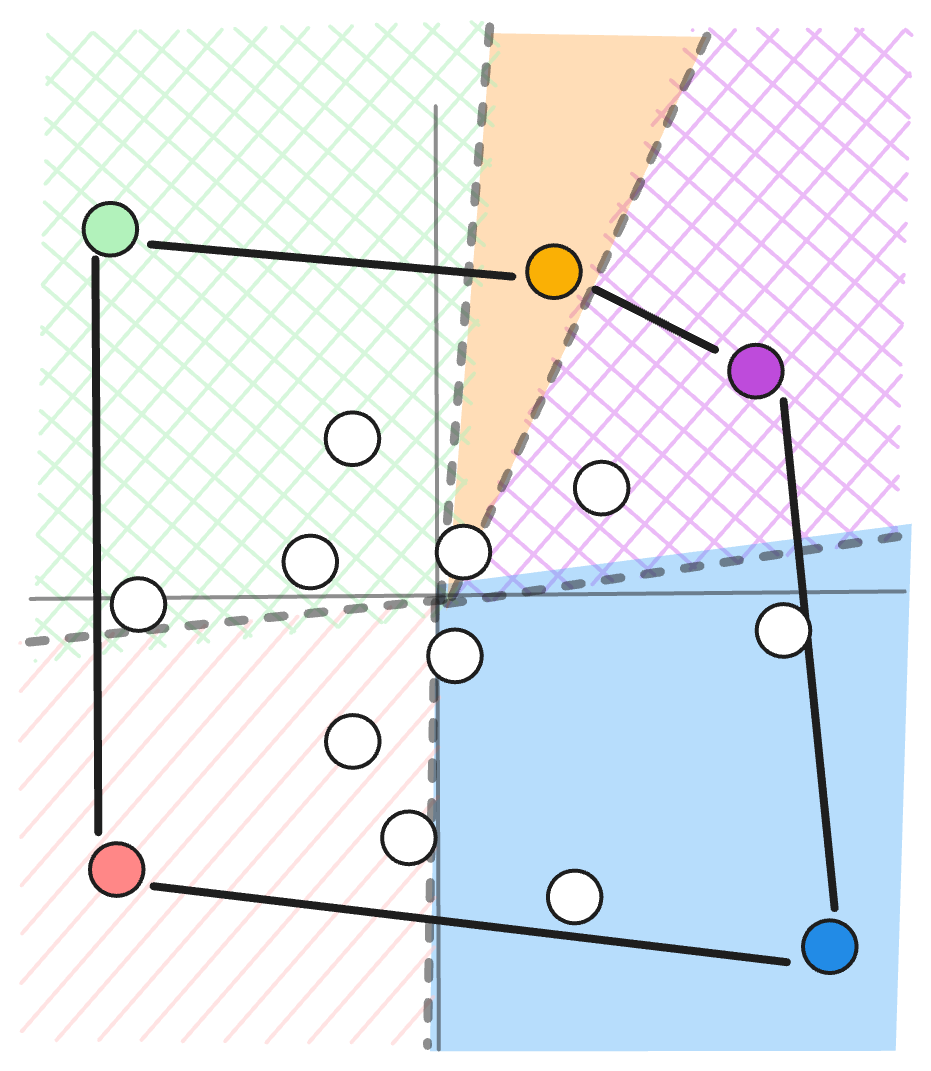
\includegraphics[width=0.32\linewidth]{figures/graphs-ip-delaunay-graph-overlay.png}
    }
    \caption{Comparison of the Voronoi diagrams and Delaunay graphs for the same set of
    points but according to Euclidean distance versus inner product. Note that, for the non-metric
    distance function based on inner product, the Voronoi regions are convex cones determined by
    the intersection of half-spaces passing through the origin. Observe additionally that the
    inner product-induced Voronoi region of a point (those in white) may be an empty set.
    Such points can never be the solution to the $1$-MIPS problem.}
    \label{figure:graphs:ip-delaunay}
\end{figure}

Moving on to the Delaunay graph,~\cite{morozov2018ip-nsw} construct the graph in much the same
way as before and call the resulting graph the IP-Delaunay graph.
Two nodes $u, v \in \mathcal{V}$ in the IP-Delaunay graph are connected if their Voronoi
regions intersect: $\mathcal{R}_u \cap \mathcal{R}_v \neq \emptyset$. Note that, by the reasoning
above, the nodes whose Voronoi regions are empty will be isolated in the graph.
These nodes represent vectors that can never be the solution to MIPS for any
query---remember that we are only considering $k=1$. So it would be inconsequential
if we removed these nodes from the graph.
This is also illustrated in Figure~\subref*{figure:graphs:ip-delaunay:ip-graph}.

Considering the data structure above for inner product,~\cite{morozov2018ip-nsw} prove the following
result to give optimality guarantee for the greedy search algorithm for $1$-MIPS
(granted we enter the graph from a non-isolated node). Nothing, however, may be said about $k$-MIPS.

\begin{theorem}
    Suppose $G=(\mathcal{V}, \mathcal{E})$ is a graph that contains the
    IP-Delaunay graph for a collection $\mathcal{X}$ minus the isolated nodes.
    Invoking Algorithm~\ref{algorithm:graphs:greedy-search} with $k=1$
    and $\delta(\cdot, \cdot) = -\langle \cdot, \cdot \rangle$
    gives the optimal solution to the top-$1$ MIPS problem.
\end{theorem}
\begin{proof}
    If we showed that a local optimum is necessarily the global optimum, then we are done.
    To that end, consider a query $q$ for which Algorithm~\ref{algorithm:graphs:greedy-search} terminates
    when it reaches node $u \in \mathcal{X}$ which is distinct from the globally optimal
    solution $u^\ast \notin N(u)$. In other words, we have that
    $\langle q, u \rangle > \langle q, v \rangle$ for all $v \in N(u)$, but
    $\langle q, u^\ast \rangle > \langle q, u \rangle$ and
    $(u, u^\ast) \notin \mathcal{E}$.
    If that is true, then $q \notin \mathcal{R}_u$, the Voronoi region of $u$,
    but instead we must have that $q \in \mathcal{R}_{u^\ast}$.

    Now define the collection $\tilde{\mathcal{X}} \triangleq N(u) \cup \{ u \}$,
    and consider the Voronoi diagram of the resulting collection. It is easy to show
    that the Voronoi region of $u$ in the presence of points in $\tilde{\mathcal{X}}$
    is the same as its region given $\mathcal{X}$. From before, we also know that $q \notin \mathcal{R}_u$.
    Considering the fact that $\mathbb{R}^d = \bigcup_{v \in \tilde{\mathcal{X}}} \mathcal{R}_v$,
    $q$ must belong to $\mathcal{R}_v$ for some $v \in \tilde{\mathcal{X}}$ with $v \neq u$.
    That implies that $\langle q, v \rangle > \langle q, u \rangle$ for some $v \in \tilde{\mathcal{X}} \setminus u$.
    But because $v \in N(u)$ (by construction), the last inequality poses a contradiction to our
    premise that $u$ was locally optimal.
\end{proof}

\medskip

In addition to the fact that the IP-Delaunay graph does not answer top-$k$ queries,
it also suffers from the same deficiencies we noted for the Euclidean Delaunay graph earlier
in this section. Naturally then, to make the data structure more practical in high-dimensional
regimes, we must resort to heuristics and approximations, which in their simplest form may be
the $k$-MIPS graph (i.e., a $k$-NN graph where the distance function for finding the top-$k$
nodes is inner product).
This is the general direction~\cite{morozov2018ip-nsw} and a few other works
have explored~\citep{Liu2019UnderstandingAI,zhou2019mobius-mips}.

As in the case of metric distance functions, none of the guarantees stated above
port over to these approximate graphs. But, once again, empirical evidence gathered from
a variety of datasets show that these graphs perform reasonably well in practice, even for top-$k$
with $k > 1$.

\subsubsection{Is the IP-Delaunay Graph Necessary?}
\cite{morozov2018ip-nsw} justify the need for developing the IP-Delaunay graph
by comparing its structure with the following alternative:
First, apply a MIPS-to-NN \emph{asymmetric} transformation~\citep{xbox-tree}
from $\mathbb{R}^d$ to $\mathbb{R}^{d + 1}$.
This involves transforming a data point $u$ with
$\phi_d(u) = [u; \; \sqrt{1 - \lVert u \rVert_2^2}]$ and a query point $q$
with $\phi_q(v) = [v; 0]$. Next,
construct the standard (Euclidean) Delaunay graph over the transformed vectors.

What happens if we form the Delaunay graph on the transformed collection
$\phi_d \big(\mathcal{X} \big)$? Observe the Euclidean distance between
$\phi_d(u)$ and $\phi_d(v)$ for two vectors $u, v \in \mathcal{X}$:
\begin{align*}
    \lVert \phi_d(u) - \phi_d(v) \rVert_2^2 &=
        \lVert \phi_d(u) \rVert_2^2 + \lVert \phi_d(v) \rVert_2^2 - 2 \langle \phi_d(u), \phi_d(v) \rangle \\
    &= \big( \lVert u \rVert_2^2 + 1 - \lVert u \rVert_2^2 \big) +
        \big( \lVert v \rVert_2^2 + 1 - \lVert v \rVert_2^2 \big) \\
        &\quad - 2\langle u, v \rangle -
        2 \sqrt{\big( 1 - \lVert u \rVert_2^2 \big) \big( 1 - \lVert v \rVert_2^2 \big)}.
\end{align*}
Should we use these distances to construct the Delaunay graph, the resulting
structure will have nothing to do with the original MIPS problem.
That is because the $L_2$ distance between a pair of transformed data points
is not rank-equivalent to the inner product between the original data points.
For this reason,~\cite{morozov2018ip-nsw} argue that the IP-Delaunay graph is a more
sensible choice.

However, we note that their argument rests heavily on their particular choice of
MIPS-to-NN transformation. The transformation they chose makes sense in
contexts where we \emph{only} care about preserving the inner product between query-data
point pairs. But when forming the Delaunay graph, preserving inner product between pairs of
data points, too, is imperative. That is the reason why we lose rank-equivalence
between $L_2$ in $\mathbb{R}^{d+1}$ and inner product in $\mathbb{R}^d$.

There are, in fact, MIPS-to-NN transformations that are more appropriate for this problem
and would invalidate the argument for the need for the IP-Delaunay graph.
Consider for example $\phi_d: \mathbb{R}^d \rightarrow \mathbb{R}^{d + m}$ for a collection
$\mathcal{X}$ of $m$ vectors as follows:
$\phi_d(u^{(i)}) = u^{(i)} \oplus \big(\sqrt{1 - \lVert u^{(i)} \rVert_2^2}\big) e_{(d + i)}$,
where $u^{(i)}$ is the $i$-th data point in the collection, and
$e_j$ is the $j$-th standard basis vector. In other words, the $i$-th $d$-dimensional
data point is augmented with an $m$-dimensional
sparse vector whose $i$-th coordinate is non-zero.
The query transformation is simply $\phi_q(q) = q \oplus \mathbf{0}$, where $\mathbf{0} \in \mathbb{R}^m$
is a vector of $m$ zeros.

Despite the dependence on $m$, the transformation is remarkably easy to manage:
the sparse subspace of every vector has at most one non-zero coordinate,
making the doubling dimension of the sparse subspace $\mathcal{O}(\log m)$
by Lemma~\ref{lemma:intrinsic-dimensionality:sparse}.
Distance computation between the transformed vectors, too, has negligible overhead.
Crucially, we regain rank-equivalence between $L_2$ distance in $\mathbb{R}^{d + m}$
and inner product in $\mathbb{R}^d$ not only for query-data point pairs, but also
for pairs of data points:
\begin{align*}
    \lVert \phi_d(u) - \phi_d(v) \rVert_2^2 &=
        \lVert \phi_d(u) \rVert_2^2 + \lVert \phi_d(v) \rVert_2^2 - 2 \langle \phi_d(u), \phi_d(v) \rangle \\
    &= 2 - 2\langle u, v \rangle.
\end{align*}

Finally, unlike the IP-Delaunay graph, the standard Delaunay graph in $\mathbb{R}^{d + m}$
over the transformed vector collection has optimality guarantee for the 
top-$k$ retrieval problem per Theorem~\ref{theorem:graphs:delaunay:top-k}.
It is, as such, unclear if the IP-Delaunay graph is even necessary as a theoretical tool.

\begin{svgraybox}
    In other words, suppose we are given a collection of points $\mathcal{X}$
    and inner product as the similarity function. Consider a graph index where
    the presence of an edge is decided based on the inner product between data points.
    Take another graph index built for the transformed $\mathcal{X}$
    using the transformation described above from $\mathbb{R}^d$ to $\mathbb{R}^{d + m}$,
    and where the edge set is formed on the basis of the Euclidean distance between two
    (transformed) data points. The two graphs are equivalent.

    The larger point is that, MIPS over $m$ points in $\mathbb{R}^d$ is equivalent
    to NN over a transformation of the points in $\mathbb{R}^{d + m}$.
    While the transformation increases the apparent dimensionality,
    the intrinsic dimensionality of the data only increases by $\mathcal{O}(\log m)$.
\end{svgraybox}

\section{The Small World Phenomenon}
Consider, once again, the Delaunay graph but, for the moment, set aside
the fact that it is a prohibitively-expensive data structure to maintain for
high dimensional vectors. By construction, every node in the graph is only
connected to its Voronoi neighbors (i.e., nodes whose Voronoi region intersects
with the current node's). We showed that such a topology affords \emph{navigability},
in the sense that the greedy procedure in Algorithm~\ref{algorithm:graphs:greedy-search}
can traverse the graph only based on information about immediate neighbors of a node
and yet arrive at the globally optimal solution to the top-$k$ retrieval problem.

\begin{svgraybox}
Let us take a closer look at the traversal algorithm for the case of $k=1$.
It is clear that, navigating from the entry node to the solution takes us through
every Voronoi region along the path. That is, we cannot ``skip'' a Voronoi region
that lies between the entry node and the answer. This implies that the running time
of Algorithm~\ref{algorithm:graphs:greedy-search} is directly affected by the diameter
of the graph (in addition to the average degree of nodes).
\end{svgraybox}

Can we enhance this topology by adding \emph{long-range} edges between non-Voronoi
neighbors, so that we may skip over a fraction of Voronoi regions? After all,
Theorem~\ref{theorem:graphs:delaunay:top-k} guarantees navigability so long as the graph
\emph{contains} the Delaunay graph. Starting with the Delaunay graph and inserting
long-range edges, then, will not take away any of the guarantees.
But, what is the right number of long-range edges and how do we determine
which remote nodes should be connected? This section reviews the theoretical results
that help answer these questions.

\begin{figure}[t]
    \centering
    \centering
    \subfloat[]{
        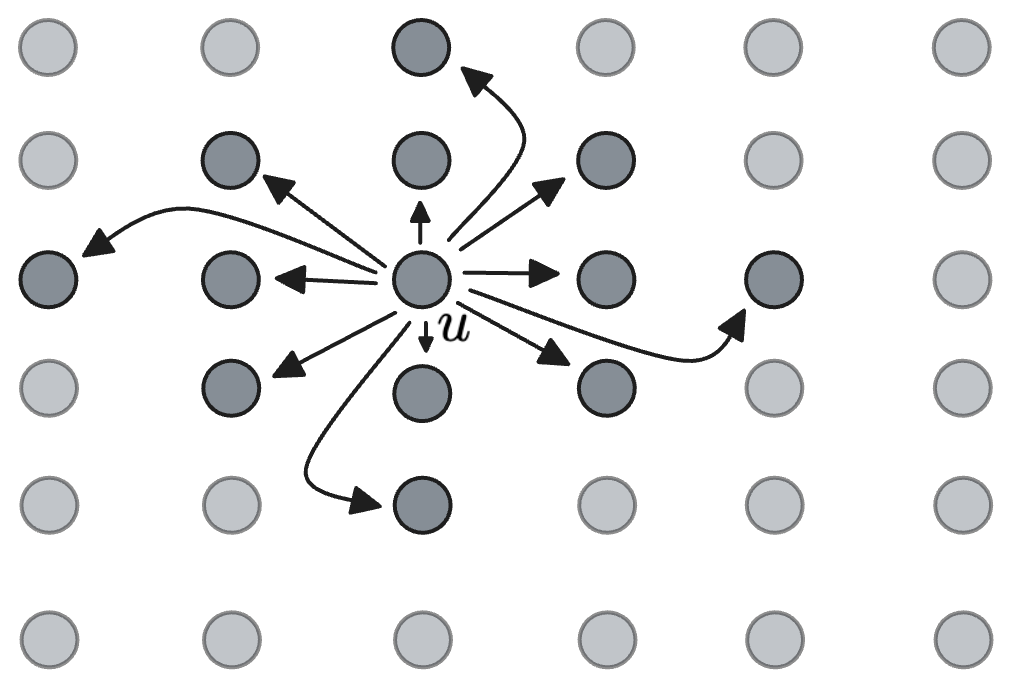
\includegraphics[width=0.35\linewidth]{figures/graphs-sw-lattice-local.png}
    }
    \hspace{2em}
    \subfloat[]{
        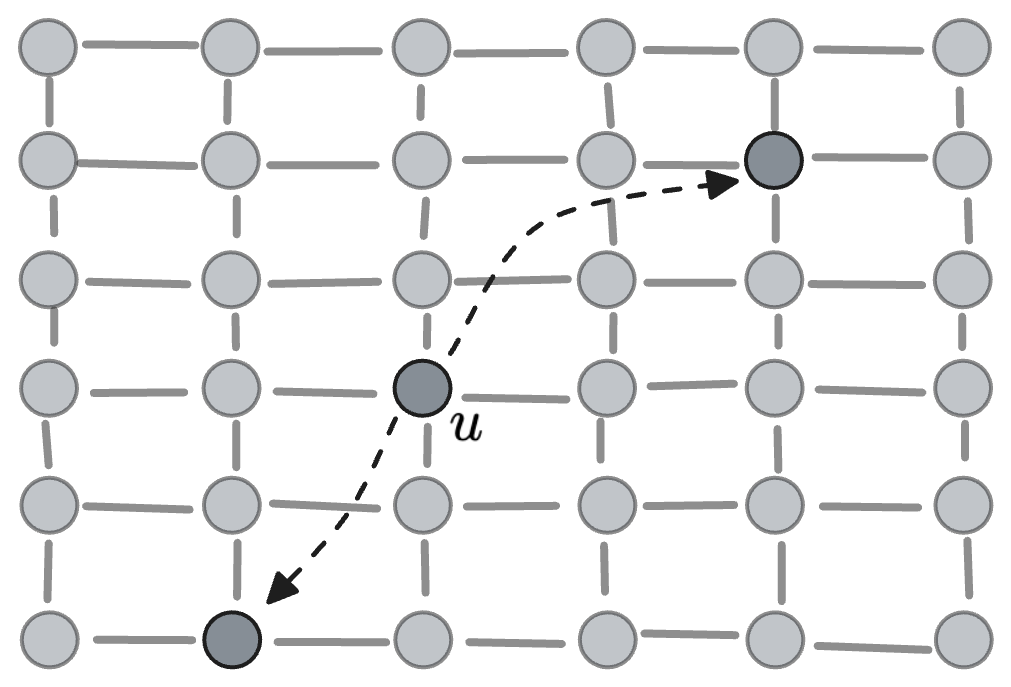
\includegraphics[width=0.35\linewidth]{figures/graphs-sw-lattice-long-range.png}
    }
    \caption{Example graphs generated by the probabilistic model introduced
    by~\cite{kleinberg2000sw}. (a) illustrates the directed edges from $u$ for
    the following configuration: $r = 2$, $l = 0$. (b) renders the regular
    structure for $r=1$, where edges without arrows are bi-directional,
    and the long-range edges for node $u$ with configuration $l=2$.}
    \label{figure:graphs:lattice}
\end{figure}

\subsection{Lattice Networks}
Let us begin with a simple topology that is relatively easy to reason
about---we will see later how the results from this section can be generalized to the Delaunay graph.
The graph we have in mind is a lattice network where $m \times m$
nodes are laid on a two-dimensional grid.
Define the distance between two nodes as their \emph{lattice (Manhattan) distance}
(i.e., the minimal number of horizontal and vertical hops that connect two nodes).
That is the network examined by~\cite{kleinberg2000sw} in a seminal paper
that studied the effect of long-range edges on the time complexity of
Algorithm~\ref{algorithm:graphs:greedy-search}.

We should take a brief detour and note that,~\cite{kleinberg2000sw},
in fact, studied the problem of \emph{transmitting}
a message from a source to a known target using the best-first-search algorithm,
and quantified the average number
of hops required to do that in the presence of a variety of classes of
long-range edges. That, in turn, was inspired by a social phenomenon
colloquially known as the ``small-world phenomenon'': The empirical observation
that two strangers are linked by a short chain of
acquaintances~\citep{milgram_small-world_1967,travers1969sw}.

In particular,~\cite{kleinberg2000sw} was interested in explaining why
and under what types of long-range edges should our greedy algorithm
be able to navigate to the optimal solution, by only utilizing information
about immediate neighbors. To investigate this question,~\cite{kleinberg2000sw}
introduced the following probabilistic model of the lattice topology as an abstraction
of individuals and their social connections.

\subsubsection{The Probabilistic Model}
Every node in the graph has a (directed) edge with every other node within
lattice distance $r$, for some fixed hyperparameter $r \geq 1$. These connections
make up the regular structure of the graph. Overlaid with this structure is a set of
random, long-range edges that are generated according to the following
probabilistic model. For fixed constants $l \geq 0$ and $\alpha \geq 0$,
we insert a directed edge between every node $u$ and $l$ other nodes, where a node
$v \neq u$ is selected with probability proportional to $\delta(u, v)^{-\alpha}$
where $\delta(u, v) = \lVert u - v \rVert_1$ is the lattice distance.
Example graphs generated by this process are depicted in Figure~\ref{figure:graphs:lattice}.

The model above is reasonably powerful as it can express a variety of topologies.
For example, when $l = 0$, the resulting graph has no long-range edges.
When $l > 0$ and $\alpha = 0$, then every node $v \neq u$ in the graph
has an equal chance of being the destination of a long-range edge from $u$.
When $\alpha$ is large, the protocol becomes more biased to forming a long-range connection
from $u$ to nodes closer to it.

\subsubsection{The Claim}
\begin{svgraybox}
\cite{kleinberg2000sw} shows that, when $0 \leq \alpha < 2$,
the best-first-search algorithm must visit at least $\mathcal{O}_{r, l, \alpha}\big(m^{(2 - \alpha)/3}\big)$
nodes. When $\alpha > 2$, the number of nodes visited is at least
$\mathcal{O}_{r, l, \alpha}\big(m^{(\alpha - 2)/(\alpha - 1)} \big)$ instead. But, rather
uniquely, when $\alpha = 2$ and $r = l = 1$, we visit a number of nodes that
is at most poly-logarithmic in $m$.
\end{svgraybox}

Theorem~\ref{theorem:graphs:lattice} states this result formally.
But before we present the theorem, we state a useful lemma.

\begin{lemma}
    \label{lemma:graphs:lattice}
    Generate a lattice $G = (\mathcal{V}, \mathcal{E})$ of $m \times m$
    nodes using the probabilistic model above
    with $\alpha = 2$ and $l = 1$.
    The probability that there exists a long-range edge between two nodes
    $u, v \in \mathcal{V}$ is at least $\delta(u, v)^{-2} / 4 \ln(6m)$.
\end{lemma}
\begin{proof}
    $u$ chooses $v \neq u$ as its long-range destination
    with the following probability: $\delta(u, v)^{-2} / \sum_{w \neq u} \delta(u, w)^{-2}$.
    Let us first bound the denominator as follows:
    \begin{align*}
        \sum_{w \neq u} \delta(u, w)^{-2} &\leq \sum_{i = 1}^{2m - 2} (4i)(i^{-2})
        = 4 \sum_{i = 1}^{2m - 2} \frac{1}{j} \\
        &\leq 4 + 4 \ln \big( 2m - 2 \big) \leq 4 \ln \big( 6m \big).
    \end{align*}
    In the expression above, we derived the first inequality by iterating over
    all possible (lattice) distances between $m^2$ nodes on a two-dimensional grid
    (ranging from $1$ to $2m - 2$ if $u$ and $w$ are at diagonally opposite corners),
    and noticing that there are at most $4i$ nodes at distance $i$ from node $u$.
    From this we infer that the probability that node $(u, v) \in \mathcal{E}$ is at least
    $\delta(u, v)^{-2} / 4 \ln(6m)$.
\end{proof}

\begin{theorem}
    \label{theorem:graphs:lattice}
    Generate a lattice $G = (\mathcal{V}, \mathcal{E})$ of $m \times m$
    nodes using the probabilistic model above
    with $\alpha = 2$ and $r = l = 1$.
    The best-first-search algorithm beginning from any arbitrary node
    and ending in a target node visits at most $\mathcal{O}\big( \log^2 m \big)$ nodes on average.
\end{theorem}
\begin{proof}
    Define a sequence of sets $A_i$, where each $A_i$ consists of nodes whose distance
    to the target $u^\ast$ is greater than $2^i$ and at most $2^{i + 1}$.
    Formally, $A_i = \{ v \in \mathcal{V} \;|\; 2^i < \delta(u^\ast, v) \leq 2^{i + 1} \}$.
    Suppose that the algorithm is currently in node $u$
    and that $\log m \leq \delta(u, u^\ast) < m$, so that $u \in A_i$
    for some $\log \log m \leq i < \log m$. What is the probability that the algorithm
    exits the set $A_i$ in the next step?
    
    That happens when one of $u$'s neighbors has a distance to $u^\ast$ that is
    at most $2^i$. In other words, $u$ must have a neighbor that is in the set
    $A_{<i} = \cup_{j=0}^{j=i-1} A_j$.
    The number of nodes in $A_{<i}$ is at least:
    \begin{equation*}
        1 + \sum_{s=1}^{2^i} s = 1 + \frac{2^i \big( 2^i + 1\big)}{2} > 2^{2i - 1}.
    \end{equation*}

    How likely is it that $(u, v) \in \mathcal{E}$ if $v \in A_{<i}$?
    We apply Lemma~\ref{lemma:graphs:lattice}, noting that the distance of each of the
    nodes in $A_{<i}$ with $u$ is at most $2^{i + 1} + 2^i < 2^{i + 2}$.
    We obtain that, the probability that $u$ is connected to a node in $A_{<i}$ is at least
    $2^{2i - 1} (2^{i + 2})^{-2} / 4 \ln(6m) = 1 / 128 \ln (6m)$.

    Next, consider the total number of nodes in $A_i$ that are visited by the algorithm,
    and denote it by $X_i$. In expectation, we have the following:
    \begin{equation*}
        \ev \big[ X_i \big] = \sum_{j = 1}^\infty \probability \big[ X_i \geq j \big] \leq
        \sum_{j = 1}^\infty \Big( 1 - \frac{1}{128 \ln (6m)} \Big)^{j - 1} =
        128 \ln (6m).
    \end{equation*}
    We obtain the same bound if we repeat the arguments for $i = \log m$.
    When $0 \leq i < \log \log m$, the algorithm visits at most $\log m$
    nodes, so that the bound above is trivially true.

    Denoting by $X$ the total number of nodes visited, $X = \sum_{j = 0}^{\log m} X_j$,
    we conclude that:
    \begin{equation*}
        \ev \big[ X \big] \leq (1 + \log m)(128 \ln(6m)) = \mathcal{O}(\log^2 m),
    \end{equation*}
    thereby completing the proof.
\end{proof}

The argument made by~\cite{kleinberg2000sw} is that, in a lattice network
where each node is connected to its (at most four) nearest neighbors within
unit distance, and where every node has a long-range edge to one other node
with probability that is proportional to $1/\delta(\cdot, \cdot)^2$, then
the greedy algorithm visits at most a poly-logarithmic number of nodes.
Translating this result to the case of top-$1$ retrieval using
Algorithm~\ref{algorithm:graphs:greedy-search} over the same network,
we can state that
the time complexity of the algorithm is $\mathcal{O}(\log^2 m)$,
because the total number of neighbors per node is $\mathcal{O}(1)$.

While this result is significant, it only holds for the lattice network
with the lattice distance. It has thus no bearing on the time complexity of
top-$1$ retrieval over the Delaunay graph with the Euclidean distance.
In the next section, we will see how~\cite{voronet2007} close this gap.

\subsection{Extension to the Delaunay Graph}
We saw in the preceding section that, the secret to creating a 
provably navigable graph where the best-first-search algorithm
visits a poly-logarithmic number of nodes in the lattice network, was the
highly specific distribution from which long-range edges were sampled.
That element turns out to be the key ingredient when extending
the results to the Delaunay graph too, as~\cite{voronet2007} argue.

We will describe the algorithm for data in the two-dimensional unit square.
That is, we assume that the collection of data points $\mathcal{X}$
and query points are in $[0, 1]^2$.
That the vectors are bounded is not a limitation \emph{per se}---as we discussed previously,
we can always normalize vectors into the hypercube without loss of generality.
That the algorithm does not naturally extend to high dimensions is a serious
limitation, but then again, that is not surprising considering the Delaunay graph
is expensive to construct. However, in the next section, we will review
heuristics that take the idea to higher dimensions.

\subsubsection{The Probabilistic Model}
Much like the lattice network, we assume there is a base graph
and a number of randomly generated long-range edges between nodes.
For the base graph,~\cite{voronet2007}
take the Delaunay graph.\footnote{\cite{voronet2007} additionally
connect all nodes that are within
$\delta_\textsc{Min} \propto 1/m$ distance from each
other, where $\delta_\textsc{Min}$ is chosen
such that the expected number of uniformly-distributed points in a
ball of radius $\delta_\textsc{Min}$ is $1$. We reformulate their method
without $\delta_\textsc{Min}$ in the present monograph to simplify
their result.}
As for the long-range edges, each node has a directed edge to one other node
that is selected at random, following a process we will describe shortly.
Observe that in this model, the number of neighbors of each node is $\mathcal{O}(1)$.

We already know from Theorem~\ref{theorem:graphs:delaunay:top-k} that,
because the network above contains the Delaunay graph, it is navigable by Algorithm~\ref{algorithm:graphs:greedy-search}. What remains to be investigated
is what type of long-range edges could reduce the number of hops (i.e.,
the number of nodes the algorithm must visit as it navigates
from an entry node to a target node).
Because at each hop the algorithm needs to evaluate distances with $\mathcal{O}(1)$
neighbors, improving the number of steps directly improves the time complexity
of Algorithm~\ref{algorithm:graphs:greedy-search} (for the case of $k=1$).

\begin{figure}[t]
    \centering
    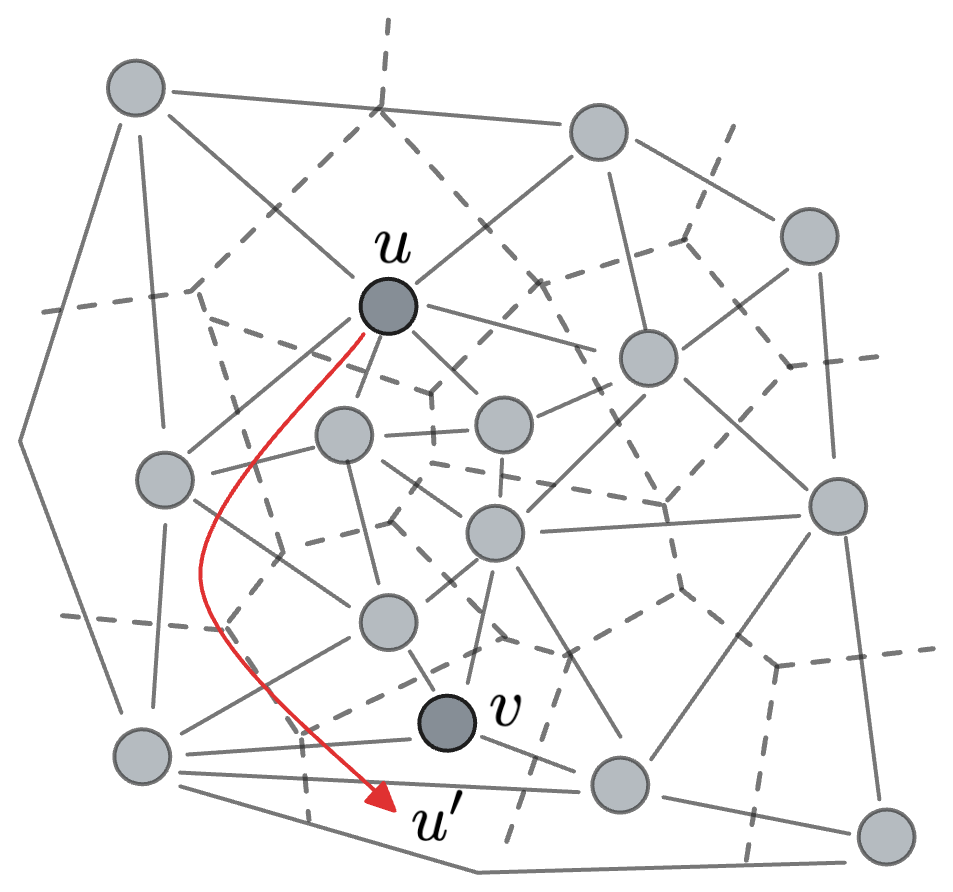
\includegraphics[width=0.35\linewidth]{figures/graphs-voronet.png}
    \caption{Formation of a long-range edge from $u$ to $v$ by the probabilistic
    model of~\cite{voronet2007}. First, we jump from $u$ to a random long-range end-point $u^\prime$,
    then designate its nearest neighbor ($v$) as the target of the edge.}
    \label{figure:graphs:voronet}
\end{figure}

\cite{voronet2007} show that, if long-range edges are chosen according to
the following protocol, then the number of hops is poly-logarithmic in $m$.
The protocol is simple: For a node $u$ in the graph,
first sample $\alpha$ uniformly from $[\ln \delta^\ast, \ln \delta_\ast]$,
where $\delta^\ast = \min_{v, w \in \mathcal{X}} \delta(v, w)$
and $\delta_\ast = \max_{v, w \in \mathcal{X}} \delta(v, w)$.
Then choose $\theta \sim [0, 2\pi]$, to finally obtain $u^\prime = u + z$
where $z$ is the vector $[e^\alpha \cos \theta, e^\alpha \sin \theta]$.
Let us refer to $u^\prime$ as the
``long-range end-point,'' and note that this point may escape
the $[0, 1]^2$ square. Next, we find the nearest node $v$ to $u^\prime$
and add a directed edge from $u$ to $v$.
This is demonstrated in Figure~\ref{figure:graphs:voronet}.

\subsubsection{The Claim}

Given the resulting graph,~\cite{voronet2007} state and prove that the
average number of hops taken by the best-first-search algorithm is poly-logarithmic.
Before we discuss the claim, however, let us state a useful lemma.

\begin{lemma}
    \label{lemma:graphs:voronet}
    The probability that the long-range end-point from a node $u$ lands in a ball
    centered at another node $v$ with radius $\beta \delta(u, v)$ for some small $\beta \in [0, 1]$
    is at least $K \beta^2 / (1 + \beta)^2$ where $K = (2 \ln \Delta)^{-1}$ and
    $\Delta = \delta_\ast / \delta^\ast$ is the aspect ratio.
\end{lemma}
\begin{proof}
    The probability that the long-range end-point lands in an area $dS$ that covers
    the distance $[r, r + dr]$ and angle $[\theta, \theta + d\theta]$, for small $dr$ and $d\theta$, is:
    \begin{equation*}
        \frac{d\theta}{2\pi} \frac{\ln (r + dr) - \ln r}{\ln \delta_\ast - \ln \delta^\ast} \approx
        \frac{d\theta}{2\pi} \frac{dr/r}{\ln \Delta} =
        \frac{1}{2\pi\ln \Delta} \frac{r d\theta dr}{r^2} \approx
        \frac{dS}{2 \pi \ln \Delta r^2}
    \end{equation*}.

    Observe now that the distance between a point $u$ and any point in the ball
    described in the lemma is at most $(1 + \beta) \delta(u, v)$. We can therefore
    see that the probability that the long-range end-point lands in $B(v, \beta \delta(u, v))$
    is at least:
    \begin{equation*}
        \frac{\pi \beta^2 \delta(u, v)^2}{2 \pi \ln \Delta (1 + \beta)^2 \delta(u, v)^2} =
        \frac{\beta^2}{2\ln(\Delta) (1 + \beta)^2},
    \end{equation*}
    as required.
\end{proof}

\begin{theorem}
    \label{theorem:graphs:voronet}
    Generate a graph $G = (\mathcal{V}, \mathcal{E})$ according to the probabilistic
    model described above, for vectors in $[0, 1]^2$ equipped with the
    Euclidean distance $\delta(\cdot, \cdot)$.
    The number of nodes visited by the best-first-search algorithm
    starting from any arbitrary node and ending at a target node is $\mathcal{O}(\log^2 \Delta)$.
\end{theorem}
\begin{proof}
    The proof follows the same reasoning as in the proof of Theorem~\ref{theorem:graphs:lattice}.

    Suppose we are currently at node $u$ and that $u^\ast$ is our target node.
    By Lemma~\ref{lemma:graphs:voronet}, the probability that the long-range end-point
    of $u$ lands in $B(u^\ast, \delta(u, u^\ast)/6)$ is at least $1/98 \ln \Delta$.
    As such, the total number of hops, $X$, from $u$ to a point in $B(u^\ast, \delta(u, u^\ast)/6)$
    has the following expectation:
    \begin{equation*}
        \ev [ X ] = \sum_{i = 1}^{\infty} \probability [X \geq i] \leq
        \sum_{i = 1}^\infty \Big( 1 - \frac{1}{98 \ln \Delta} \Big)^{i - 1} = 98 \ln \Delta.
    \end{equation*}
    Every time the algorithm moves from the current node $u$ to some other node in
    $B(u^\ast, \delta(u, u^\ast)/6)$, the distance is shrunk by a factor of $6/5$.
    As such, the total number of hops in expectation is at most:
    \begin{equation*}
        \Big( \ln_{6/5} \Delta \Big) \times \Big( 98 \ln \Delta \Big) = \mathcal{O}(\log^2 \Delta).
    \end{equation*}
\end{proof}

We highlight that,~\cite{voronet2007} choose the interval from which $\alpha$
is sampled differently. Indeed, $\alpha$ in their work is chosen uniformly from
the range $\delta_\textsc{Min} \propto 1/m$ and $\sqrt{2}$.
Substituting that configuration into Theorem~\ref{theorem:graphs:voronet} gives
an expected number of hops that is $\mathcal{O}(\log^2 m)$.

\subsection{Approximation}
The results of~\cite{voronet2007} are encouraging. In theory, so long as
we can construct the Delaunay graph, we not only have the optimality guarantee,
but we are also guaranteed to have a poly-logarithmic number of hops to
reach the optimal answer. Alas, as we have discussed previously, the Delaunay
graph is expensive to build in high dimensions.

\begin{svgraybox}
Moreover, the number of
neighbors per node is no longer $\mathcal{O}(1)$. So even if we inserted
long-range edges into the Delaunay graph, it is not immediate if the time
saved by skipping Voronoi regions due to long-range edges
offsets the additional time the algorithm
spends computing distances between each node along the path and its neighbors.
\end{svgraybox}

We are back, then, to approximation with the help of heuristics.
\cite{raynet2007} describe one such method in a follow-up study.
Their method approximates the Voronoi regions of every node by
resorting to a \emph{gossip} protocol. In this procedure, every node
has a list of $3d + 1$ of its current neighbors, where $d$ denotes the dimension
of the space. In every iteration of the algorithm,
every node passes its current list to its neighbors. When a node receives
this information, it takes the union of all lists, and finds the subset of
$3d + 1$ points with the minimal volume. This subset becomes the node's
current list of neighbors. While a na\"ive implementation of the protocol
is prohibitively expensive,~\cite{raynet2007} discuss an alternative to estimating
the volume induced by a set of $3d + 1$ points, and the search for the minimal volume.

\cite{nsw2014} take a different approach. They simply permute the vectors
in the collection $\mathcal{X}$, and sequentially add each vector to the graph. Every time
a vector is inserted into the graph, it is linked to its $k$ nearest neighbors
from the current snapshot of the graph.
The intuition is that, as the graph grows, the edges added earlier in the evolution
of the graph serve as long-range edges in the final graph,
and the more recent edges form an approximation
of the $k$-NN graph, which itself is an approximation of the Delaunay graph.
Later~\cite{hnsw2020} modify the algorithm by introducing a hierarchy of graphs.
The resulting graph has proved successful in practice and, despite its lack
of theoretical guarantees, is both effective and highly efficient.

\section{Neighborhood Graphs}

In the preceding section, our starting point was the Delaunay graph. We augmented it with
random long-range connections to improve the transmission rate through the network.
Because the resulting structure contains the Delaunay
graph, we get the optimality guarantee of Theorem~\ref{theorem:graphs:delaunay:top-k}
for free. But, as a result of the complexity of the Delaunay construction in high dimensions,
we had to approximate the structure instead, losing all guarantees in the process.
Frustratingly, the approximate structure obtained by the heuristics we discussed, is
certainly not a super-graph of the Delaunay graph, nor is it necessarily its sub-graph.
In fact, even the fundamental property of connectedness is not immediately guaranteed.
There is therefore nothing meaningful to say about the theoretical behavior of such graphs.

In this section, we do the opposite. Instead of adding edges to the Delaunay graph and
then resorting to heuristics to create a completely different graph,
we prune the edges of the Delaunay graph to find a structure that is its \emph{sub-graph}.
Indeed, we cannot say anything meaningful about the optimality of
\emph{exact} top-$k$ retrieval, but as we will later see, we can state formal results
for the approximate top-$k$ retrieval variant---albeit in a very specific case.
The structure we have in mind is known as the Relative Neighborhood
Graph (RNG)~\citep{Toussaint1980rng,relativeNeighborhoodGraphs}.

\begin{svgraybox}
In an RNG, $G = (\mathcal{V}, \mathcal{E})$, for a distance function $\delta(\cdot, \cdot)$,
there is an undirected edge between two nodes $u, v \in \mathcal{V}$ if and only if
$\delta(u, v) < \max \big( \delta(u, w), \delta(w, v) \big)$ for all
$w \in \mathcal{V} \setminus \{ u, v\}$.
That is, the graph guarantees that, if $(u, v) \in \mathcal{E}$, then there is no other
point in the collection that is simultaneously closer to $u$ and $v$, than $u$ and $v$ are to
each other. Conceptually, then, we can view constructing an RNG as pruning away
edges in the Delaunay graph that violate the RNG property.
\end{svgraybox}

The RNG was shown to contain the Minimum Spanning Tree~\citep{Toussaint1980rng},
so that it is guaranteed to be connected.
It is also provably contained in the Delaunay graph~\citep{OROURKE1982} in any metric
space and in any number of dimensions.
As a final property, it is not hard to see that such a graph $G$ comes with a weak
optimality guarantee for the best-first-search algorithm:
If $q = u^\ast \in \mathcal{X}$, then the greedy traversal algorithm
returns the node associated with $q$, no matter where it enters the graph.
That is due simply to the following fact: If the current node $u$ is a local optimum
but not the global optimum, then there must be an edge connecting $u$ to a node
that is closer to $u^\ast$. Otherwise, $u$ itself must be connected to $u^\ast$.

Later,~\cite{arya1993sng} proposed a \emph{directed} variant of the RNG,
which they call the \emph{Sparse Neighborhood Graph} (SNG) that is arguably
more suitable for top-$k$ retrieval.
For every node $u \in \mathcal{V}$, we apply the following procedure:
Let $\mathcal{U} = \mathcal{V} \setminus \{ u \}$.
Sort the nodes in $\mathcal{U}$ in increasing distance to $u$.
Then, remove the closest node (say, $v$) from $\mathcal{U}$ and add an edge between $u$ to $v$.
Finally, remove from $\mathcal{U}$ all nodes $w$ that satisfy $\delta(u, w) > \delta(w, v)$.
The process is repeated until $\mathcal{U}$ is empty.
It can be immediately seen that the weak optimality guarantee from before still holds in the SNG.

\medskip

Neighborhood graphs are the backbone of many graph algorithms for top-$k$
retrieval~\citep{nsw2014,hnsw2020,fanng2016,fu2019nsg,fu2022nssg,diskann}.
While many of these algorithms make for efficient methods in practice, the
Vamana construction~\citep{diskann} stands out as it introduces a novel
super-graph of the SNG that turns out to have provable theoretical properties.
That super-graph is what~\cite{indyk2023worstcase}
call an \emph{$\alpha$-shortcut reachable} SNG, which we will review next.
For brevity, though, we call this graph simply $\alpha$-SNG.

\begin{figure}[t]
    \centering
    \subfloat[$\alpha = 1$]{
        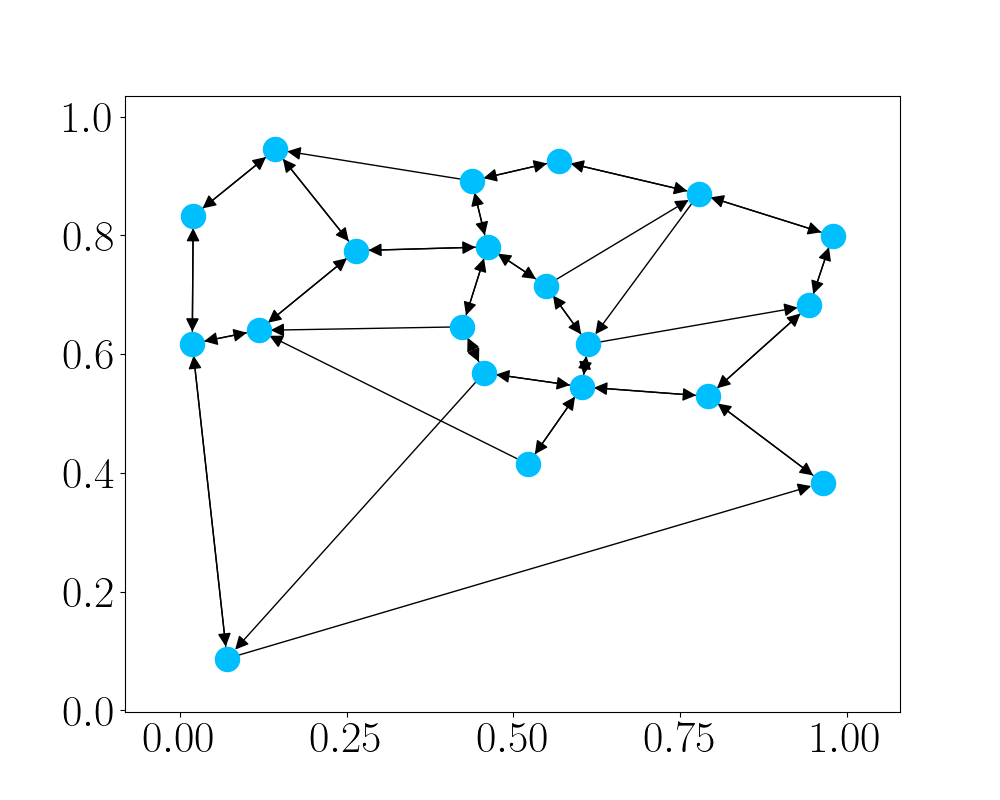
\includegraphics[width=0.45\linewidth]{figures/graphs-sng.png}
    }
    \subfloat[$\alpha = 1.1$]{
        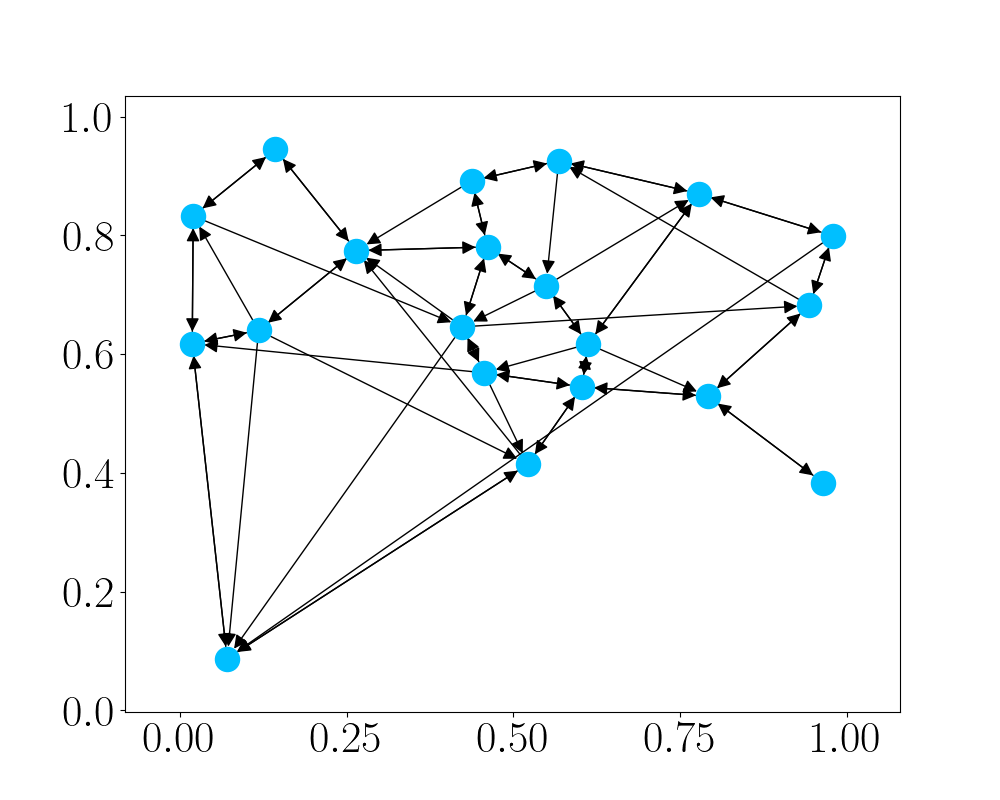
\includegraphics[width=0.45\linewidth]{figures/graphs-sng-alpha1.1.png}
    }
    
    \subfloat[$\alpha = 1.2$]{
        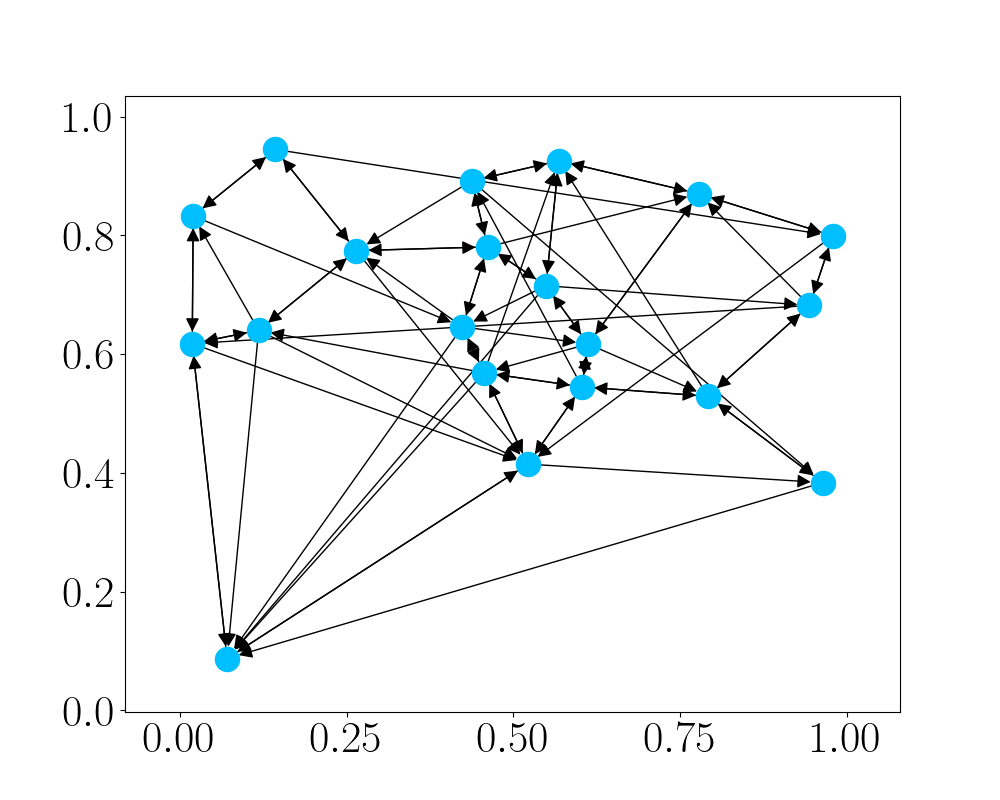
\includegraphics[width=0.45\linewidth]{figures/graphs-sng-alpha1.2.png}
    }
    \subfloat[$\alpha = 1.3$]{
        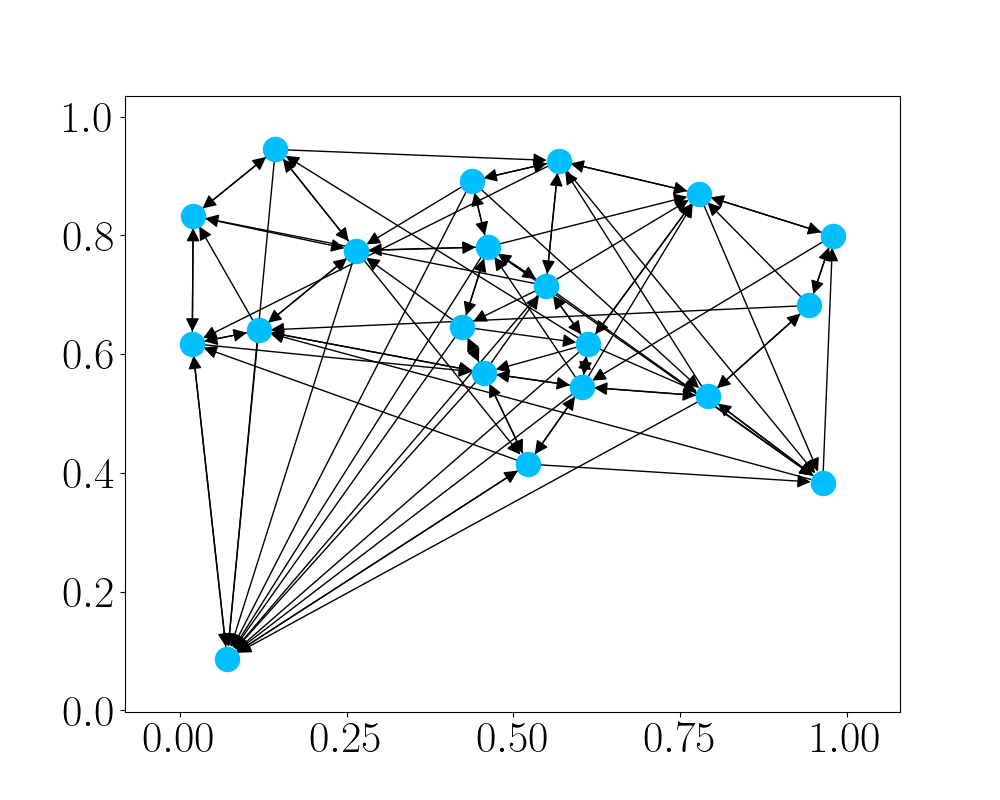
\includegraphics[width=0.45\linewidth]{figures/graphs-sng-alpha1.3.png}
    }
    \caption{Examples of $\alpha$-SNGs on a dataset of $20$ points drawn uniformly
    from $[0, 1]^2$ (blue circles).
    When $\alpha=1$, we recover the standard SNG. As $\alpha$ becomes larger, the
    resulting graph becomes more dense.}
    \label{figure:graphs:sng}
\end{figure}

\subsection{From SNG to \texorpdfstring{$\alpha$}{alpha}-SNG}
\cite{diskann} introduce a subtle adjustment to the SNG construction.
In particular, suppose we are processing a node $u$, have already extracted
the node $v$ whose distance to $u$ is minimal among the nodes in $\mathcal{U}$
(i.e., $v = \argmin_{w \in \mathcal{U}} \delta(u, w)$), and are now deciding
which nodes to discard from $\mathcal{U}$. In the standard SNG construction,
we remove a node $w$ for which $\delta(u, w) > \delta(w, v)$. But in the modified
construction, we instead discard a node $w$ if $\delta(u, w) > \alpha \delta(w, v)$
for some $\alpha > 1$. Note that, the case of $\alpha = 1$ simply gives the standard SNG.
Figure~\ref{figure:graphs:sng} shows a few examples of $\alpha$-SNGs on a toy dataset.

That is what~\cite{indyk2023worstcase} later refer to as an $\alpha$-shortcut reachable
graph. They define $\alpha$-shortcut reachability as the property where,
for any node $u$, we have that every other node $w$ is either the target of an edge
from $u$ (so that $(u, w) \in \mathcal{E}$), or that there is a node $v$
such that $(u, v) \in \mathcal{E}$ and $\delta(u, w) \geq \alpha \delta(w, v)$.
Clearly, the graph constructed by the procedure above is $\alpha$-shortcut
reachable by definition.

\subsubsection{Analysis}
\cite{indyk2023worstcase} present an analysis of the $\alpha$-SNG
for a collection of vectors $\mathcal{X}$ with \emph{doubling dimension} $d_\circ$
as defined in Definition~\ref{definition:doubling-dimension}.

For collections with a fixed doubling constant,~\cite{indyk2023worstcase} state two bounds. 
One gives a bound on the degree of every node in an $\alpha$-SNG. The other tells us
the expected number of hops from any arbitrary entry node to an $\epsilon$-approximate
solution to top-$1$ queries. The two bounds together give us an idea of the time complexity
of Algorithm~\ref{algorithm:graphs:greedy-search} over an $\alpha$-SNG as well as its
accuracy.

\begin{figure}[t]
    \centering
    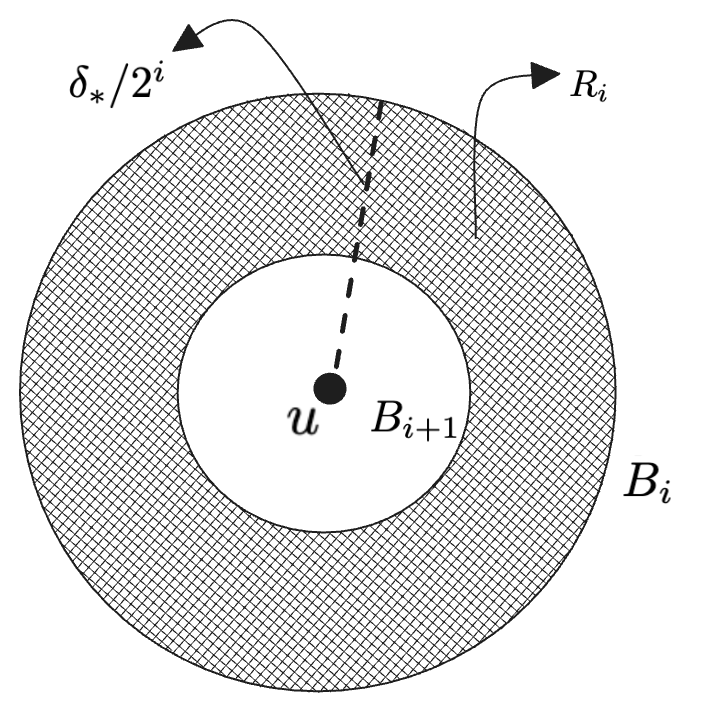
\includegraphics[width=0.3\linewidth]{figures/graphs-sng-proof.png}
    \caption{The sets $B_i$ and rings $R_i$ in the proof of Theorem~\ref{theorem:graphs:sng:degree}.}
    \label{figure:graphs:sng:proof}
\end{figure}

\begin{theorem}
    \label{theorem:graphs:sng:degree}
    The degree of any node in an $\alpha$-SNG is
    $\mathcal{O}\big( (4\alpha)^{d_\circ} \log \Delta \big)$ if the collection
    $\mathcal{X}$ has doubling dimension $d_\circ$ and aspect ratio $\Delta = \delta_\ast / \delta^\ast$.
\end{theorem}
\begin{proof}
    Consider a node $u \in \mathcal{V}$. For each $i \in [\log_2 \Delta]$, define
    a ball centered at $u$ with radius $\delta_\ast / 2^i$: $B_i = B(u, \delta_\ast / 2^i)$.
    From this, construct rings $R_i = B_i \setminus B_{i + 1}$. See Figure~\ref{figure:graphs:sng:proof}
    for an illustration.

    Because $\mathcal{X}$ has a constant doubling dimension, we can cover each $R_i$
    with $\mathcal{O}\big( (4\alpha)^{d_\circ} \big)$ balls of radius $\delta_\ast / \alpha 2^{i + 2}$.
    By construction, two points in each of these cover balls are at
    most $\delta_\ast / \alpha 2^{i + 1}$ apart. At the same time, the distance from $u$ to
    any point in a cover ball is at least $\delta_\ast / 2^{i + 1}$. By construction, all points
    in a cover ball except one are discarded as we form $u$'s edges in the $\alpha$-SNG.
    As such, the total number of edges from $u$ is bounded by the total number of cover balls,
    which is $\mathcal{O}\big( (4\alpha)^{d_\circ} \log \Delta \big)$.
\end{proof}

\begin{theorem}
    If $G = (\mathcal{V}, \mathcal{E})$ is an $\alpha$-SNG for collection $\mathcal{X}$,
    then Algorithm~\ref{algorithm:graphs:greedy-search} with $k = 1$ returns
    an $(\frac{\alpha + 1}{\alpha - 1} + \epsilon)$-approximate top-$1$ solution
    by visiting $\mathcal{O}\big( \log_\alpha \frac{\Delta}{(\alpha - 1)\epsilon} \big)$ nodes.
\end{theorem}
\begin{proof}
    Suppose $q$ is a query point and $u^\ast = \argmin_{u \in \mathcal{X}} \delta(q, u)$.
    Further assume that the best-first-search algorithm is currently in node $v_i$
    with distance $\delta(q, v_i)$ to the query. We make the following observations:
    \begin{itemize}
        \item By triangle inequality, we know that
        $\delta(v_i, u^\ast) \leq \delta(v_i, q) + \delta(q, u^\ast)$; and,
        \item By construction of the $\alpha$-SNG, $v_i$ is either connected to $u^\ast$
        or to another node whose distance to $u^\ast$ is shorter than $\delta(v_i, u^\ast) / \alpha$.
    \end{itemize}
    We can conclude that, the distance from $q$ to the next node the algorithm
    visits, $v_{i + 1}$, is at most:
    \begin{align*}
        \delta(v_{i+1}, q) &\leq \delta(v_{i + 1}, u^\ast) + \delta(u^\ast, q) \\
        &\leq \frac{\delta(v_i, u^\ast)}{\alpha} + \delta(u^\ast, q) \\
        &\leq \frac{\delta(v_i, q)}{\alpha} + (\alpha + 1) \delta(q, u^\ast).
    \end{align*}
    By induction, we see that, if the entry node is $s \in \mathcal{V}$:
    \begin{align*}
        \delta(v_i, q) &\leq \frac{\delta(s, q)}{\alpha^i} + (\alpha + 1) \delta(q, u^\ast) \sum_{j=1}^i \alpha^{-j} \\
        &\leq \frac{\delta(s, q)}{\alpha^i} + \frac{\alpha + 1}{\alpha - 1} \delta(q, u^\ast)
        \numberthis \label{equation:graphs:alpha-sng:hops-bound}.
    \end{align*}

    There are three cases to consider.

    \textbf{Case 1}: When $\delta(s, q) > 2 \delta_\ast$, then by triangle inequality,
    $\delta(q, u^\ast) > \delta(s, q) - \delta(s, u^\ast) > \delta(s, q) - \delta_\ast > \delta(s, q) / 2$.
    Plugging this into Equation~(\ref{equation:graphs:alpha-sng:hops-bound}) yields:
    \begin{align*}
        \delta(v_i, q) &\leq \frac{2\delta(q, u^\ast)}{\alpha^i} + \frac{\alpha + 1}{\alpha - 1} \delta(q, u^\ast) \\
        &\implies \frac{\delta(v_i, q)}{\delta(q, u^\ast)} \leq \frac{2}{\alpha^i} + \frac{\alpha + 1}{\alpha - 1}.
    \end{align*}
    As such, for any $\epsilon > 0$, the algorithm returns a $\big( \frac{\alpha + 1}{\alpha - 1} + \epsilon\big)$-approximate solution in $\log_\alpha 2/\epsilon$ steps.

    \textbf{Case 2}: $\delta(s, q) \leq 2 \delta_\ast$ and $\delta(q, u^\ast) \geq \frac{\alpha - 1}{4(\alpha + 1)}\delta^\ast$. By Equation~(\ref{equation:graphs:alpha-sng:hops-bound}), the algorithm returns a
    $\big( \frac{\alpha + 1}{\alpha - 1} + \epsilon \big)$-approximate solution as soon as $\delta(s, q)/\alpha^i < \epsilon \delta(q, u^\ast)$. So in this case:
    \begin{align*}
        \frac{\delta(v_i, q)}{\delta(q, u^\ast)} &\leq \frac{2 \delta_\ast}{\alpha^i \delta(q, u^\ast)} + \frac{\alpha + 1}{\alpha - 1} \\
        &\leq \frac{8 (\alpha + 1) \delta_\ast}{\alpha^i (\alpha - 1) \delta^\ast} + \frac{\alpha + 1}{\alpha - 1}.
    \end{align*}
    As such, the number of steps to reach the approximation level is $\log_\alpha \frac{8 (\alpha + 1) \Delta}{(\alpha - 1) \epsilon}$ which is $\mathcal{O}\big( \log_\alpha \Delta / (\alpha - 1) \epsilon \big)$.

    \textbf{Case 3}: $\delta(s, q) \leq 2 \delta_\ast$ and $\delta(q, u^\ast) < \frac{\alpha - 1}{4(\alpha + 1)}\delta^\ast$. Suppose $v_i \neq u^\ast$. Observe that: (a) $\delta(v_i, u^\ast) \geq \delta^\ast$;
    (b) $\delta(v_i, q) > \delta(q, u^\ast)$; and (c) $\delta(q, u^\ast) < \delta^\ast/2$ by assumption.
    As such, triangle inequality gives us: $\delta(v_i, q) > \delta(v_i, u^\ast) - \delta(u^\ast, q) >
    \delta^\ast - \delta^\ast/2 = \delta^\ast/2$. Together with Equation~(\ref{equation:graphs:alpha-sng:hops-bound}), we obtain:
    \begin{align*}
        \frac{\delta^\ast}{2} &\leq \delta(v_i, q) \leq \frac{2 \delta_\ast}{\alpha^i} + \frac{\delta^\ast}{4} \\
        &\implies \alpha^i \leq 8 \Delta \implies i \leq \log_\alpha 8\Delta.
    \end{align*}

    The three cases together give the desired result.
\end{proof}

In addition to the bounds above,~\cite{indyk2023worstcase} present negative results
for other major SNG-based graph algorithms by proving (via contrived examples)
linear-time lower-bounds on their performance. These results together show the
significance of the pruning parameter $\alpha$ in the $\alpha$-SNG construction.

\subsubsection{Practical Construction of $\alpha$-SNGs}
The algorithm described earlier to construct an $\alpha$-SNG for $m$ points
has $\mathcal{O}(m^3)$ time complexity. That is too expensive for even moderately
large values of $m$. That prompted~\cite{diskann} to approximate the $\alpha$-SNG
by way of heuristics.

The starting point in the approximate construction is a random $R$-regular graph:
Every node is connected to $R$ other nodes selected at random.
The algorithm then processes each node in random order as follows.
Given node $u$, it begins by searching the current snapshot of the graph for the top $L$
nodes for the query point $u$, using Algorithm~\ref{algorithm:graphs:greedy-search}.
Denote the returned set of nodes by $\mathcal{S}$. It then performs the
pruning algorithm by setting $\mathcal{U} = \mathcal{S} \setminus \{ u \}$, rather
than $\mathcal{U} = \mathcal{V} \setminus \{ u \}$.
That is the gist of the modified construction
procedure.\footnote{We have omitted minor but important details of the procedure
in our prose. We refer the interested reader to~\citep{diskann} for a description of
the full algorithm.}

Naturally, we lose all guarantees for approximate top-$k$ retrieval
as a result~\citep{indyk2023worstcase}. We do, however, obtain a more
practical algorithm instead that, as the authors show,
is both efficient and effective.

\section{Closing Remarks}

This chapter deviated from the pattern we got accustomed to so far in the monograph.
The gap between theory and practice in Chapters~\ref{chapter:branch-and-bound}
and~\ref{chapter:lsh} was narrow or none. That gap is rather wide, on the other hand,
in graph-based retrieval algorithms. Making theory work in practice required a great deal
of heuristics and approximations.

Another major departure is the activity in the respective bodies of literature.
Whereas trees and hash families have reached a certain level of maturity,
the literature on graph algorithms is still evolving, actively so.
A quick search through scholarly articles shows growing interest in this class
of algorithms. This monograph itself presented results that were obtained very recently.

There is good reason for the uptick in research activity.
Graph algorithms are among the most successful algorithms there are
for top-$k$ vector retrieval. They are often remarkably fast during retrieval
and produce accurate solution sets.

That success makes it all the more enticing to improve their other characteristics.
For example, graph indices are often large, requiring far too much memory.
Incorporating compression into graphs, therefore, is a low-hanging fruit
that has been explored~\citep{singh2021freshdiskann} but needs further investigation.
More importantly, finding an even sparser graph without losing accuracy
is key in reducing the size of the graph to begin with, and that boils down
to designing better heuristics.

Heuristics play a key role in the construction time of graph indices too.
Building a graph index for a collection of billions of points, for example,
is not feasible for the variant of the Vamana algorithm that offers theoretical
guarantees. Heuristics introduced in that work lost all such guarantees,
but made the graph more practical.

Enhancing the capabilities of graph indices too is an important practical
consideration. For example, when the graph is too large and, so, must rest
on disk, optimizing disk access is essential in maintaining the speed of
query processing~\citep{diskann}. When the collection of vectors is live
and dynamic, the graph index must naturally handle deletions and insertions
in real-time~\citep{singh2021freshdiskann}. When vectors come with metadata
and top-$k$ retrieval must be constrained to the vectors that pass
a certain set of metadata filters, then a greedy traversal of the graph
may prove sub-optimal~\citep{filtered-diskann2023}. All such questions
warrant extensive (often applied) research and go some way to make
graph algorithms more attractive to production systems.

There is thus no shortage of practical research questions.
However, the aforementioned gap between theory and practice should not
dissuade us from developing better theoretical algorithms.
The models that explained the small world phenomenon may not be directly
applicable to top-$k$ retrieval in high dimensions, but they inspired
heuristics that led to the state of the art. Finding theoretically-sound
edge sets that improve over the guarantees offered by Vamana
could form the basis for other, more successful heuristics too.

\bibliographystyle{abbrvnat}
\bibliography{biblio}
